\section{Prologue}

Here we get to the overall goal of the thesis, the determination of the formyl isomer branching ratio at temperatures relevant to the ISM. The results up to this point were, more or less, due to the need to understand the reactions that occur in the trap and how they may affect the isomer measurement. 

\section{Introduction}

The ratios of the formyl isomers \ce{HCO+} and \ce{HOC+} in the ISM vary wildly from one body to the next.\cite{Liszt2004} This can be due to isomerization of \ce{HOC+} via reactions with \ce{H2}, or the reaction channels that produce the two isomers.\cite{Apponi1997} Of the various reaction channels, we would like to find the differences between
\begin{align}
	\ce{C+ + H2O & -> HCO+ + H} \label{r: C+H2O->HCO} \\
	\ce{& -> HOC+ + H}. \label{r: C+H2O->HOC}
\end{align}
Both reactions are exothermic, by $-5.05$ eV and $-3.34$ eV, for main reactions \ref{r: C+H2O->HCO} and \ref{r: C+H2O->HOC} respectively.\cite{Chalk1997} We define the branching ratio of interest is to be the percentage \ce{HOC+} production to that of \ce{HCO+}, \ce{HOC+}:\ce{HCO+}. This ratio has been experimentally found to be 86:14 at room temperature\cite{Freeman1987}, but unknown at temperatures relevant to the ISM, where these kind of ion-dipole reactions would dominate.

By definition, these formyl isomers of reactions \cref{r: C+H2O->HCO,r: C+H2O->HOC} have identical mass and thus, cannot be readily read off by the TOF system. To be able to separate the isomer products, we need to be able to separate their masses. By introducing a gas into the system with a proton affinity in between the isomer products, we may selectively react only the less stable \ce{HOC+} isomer. This also yields a distinct $m/z$ peaks originating from separate isomers as seen in the titration reactions \ref{r: X+HOC->XH} and \ref{r: X+HCO->NR}. But by using an external gas, we are doing an indirect measurement, and as such, it may add unintended complications. We must consider if the reaction products are in a long lived internally excited state that may cause an undesired reaction, skewing the measured ratio. A concern is that certain gasses may react with the excited \ce{Be+}, \ce{C+}, or any other ionized species in the trap, possibly affecting the branching ratio measurement. Finally, since \ce{HOC+} is the less stable isomer, there is a possiblity that it can isomerize and change into the more stable \ce{HCO+}. By itself, this would not occur due to a 1.5 eV barrier, but the introduction of a gas with appropriate proton affinity may cause isomerization shown in reaction \ref{r: X+HOC->HCO}, instead of proton abstraction (reaction \ref{r: X+HOC->XH}).\cite{Chalk1997}
\begin{align}
	\ce{HOC+ + X & -> XH+ + CO} \label{r: X+HOC->XH} \\
	\ce{& -> HCO+ + X} \label{r: X+HOC->HCO} \\
	\ce{HCO+ + X & -> no reaction} \label{r: X+HCO->NR}
\end{align}

\begin{table}[H]
	\centering
	\label{tab: affinities}
	\begin{tabular}{|l|c|c|}
		\hline
		& Affinity (kJ/mol) & Affinities (eV)   \\
		\hline
		\ce{O2}  & 422 & 4.37 \\
		\ce{H2}  & 424 & 4.39 \\
		\ce{Kr}  & 425 & 4.40 \\
		\ce{CO}* & 427 & 4.43 \\
		\ce{HF}  & 490 & 5.08 \\
		\ce{N2}  & 495 & 5.13 \\
		\ce{Xe}  & 496 & 5.14 \\
		\ce{NO}  & 531 & 5.50 \\
		\ce{CO2} & 548 & 5.68 \\
		\ce{CH4} & 552 & 5.72 \\
		\ce{HCl} & 564 & 5.85 \\
		\ce{HBr} & 569 & 5.90 \\
		\ce{N2O} & 571 & 5.92 \\
		*\ce{CO} & 594 & 6.16 \\
		\hline
	\end{tabular}
	\caption{Proton affinities of gasses between formyl isomers where (*) indicates H bonding location.\cite{Johnson2018}}
\end{table}

The previous 305 K measurement of the branching ratio used a titration gas as well in a selected ion flow tube (SIFT) instrument with \ce{N2O}, while rate constants for reactions with \ce{O2}, \ce{Kr}, \ce{Xe}, \ce{CO}, \ce{CO2}, and \ce{CH4} were explored.\cite{Love1987,Freeman1987} Titration with \ce{Xe}, \ce{CO2}, \ce{CH4}, \ce{N2O}, and \ce{^15N2} were tested with varying degrees of success. Due to reactions with the trapped \ce{C+}, \ce{CH4} produced new $m/z$ peaks due to a direct reaction, as well as subsequent reactions, at which point we could not be certain the peaks of interest were due to the main reaction. The effect of \ce{N2O} onto \ce{Be+} was not known before our study, and are still not completely understood. There seem to be multiple subsequent reactions occurring because the \ce{Be+} is quickly depleted from the trap without replacement, meaning, a very heavy ion that is not stable is being produced, causing an overall loss of ions in the trap. Without the coolant ion, the mass resolution of the TOF declines significantly, to where the masses of interest start overlapping with nearby signals. With \ce{Xe}, the charged product \ce{XeH+} has a mass to charge ratio of $m/z=132$, far too heavy for the trap, meaning we would have to know exactly how much of both isomers were produced in a single run to derive a branching ratio, which was not a reliable measurement. In the end, we used a gas that was not previously used in the literature, \ce{^15N2} as it only reacts with \ce{HOC+}, while producing a new mass peak. \ce{O2} was also introduced into the chamber to not separate the isomers, but to determine if there were long lived internal states that would affect the branching ratio results.

\section{Internal Relaxation}

Through the \ce{C+ + H2O} reaction, 3.34 eV of energy is released in the production of \ce{HOC+}, while an even greater 5.05 eV for \ce{HCO+}. The released energy has two avenues, the kinetic energy of the reaction products of \ce{[HCO]+} and \ce{H}, and the internal states of the isomer produced. If the isomer is produced in a highly excited internal state, this could cause problems for our titration process if they are long lived and of high enough energy to cause the more stable \ce{HCO+} to react with a titration gas \ce{CO2H} when it would not have in its internal ground state. If \ce{HCO+} retains but 0.48 eV of the initial 5.05 eV in an internal state, it could cause the production of \ce{CO2H+}, despite not being reactive in the ground state.

To see if these internal states may be an issue, we use \ce{O2} as a titration gas. Table \ref{tab: affinities} shows that \ce{O2} is only 0.05 eV away from being able to react with the less stable \ce{HOC+}. By introducing \ce{H2O} via the general valve, and \ce{O2} from a valve behind a leak valve, the two gasses can be introduced with a well defined time delay. Mauclaire et al. found that the radiative lifetimes of these states can be as high as $\approx 300$ ms\cite{Mauclaire1995} which means a delay of 1 s between the introduction of the two gasses should be sufficient for more than 99\% of the internally excited states to have radiatively decayed, preventing any production of \ce{O2H+}. The procedure is performed and resulting TOF trace is shown in Figure \ref{fig: O2 titration}.

\begin{figure}
	\centering
	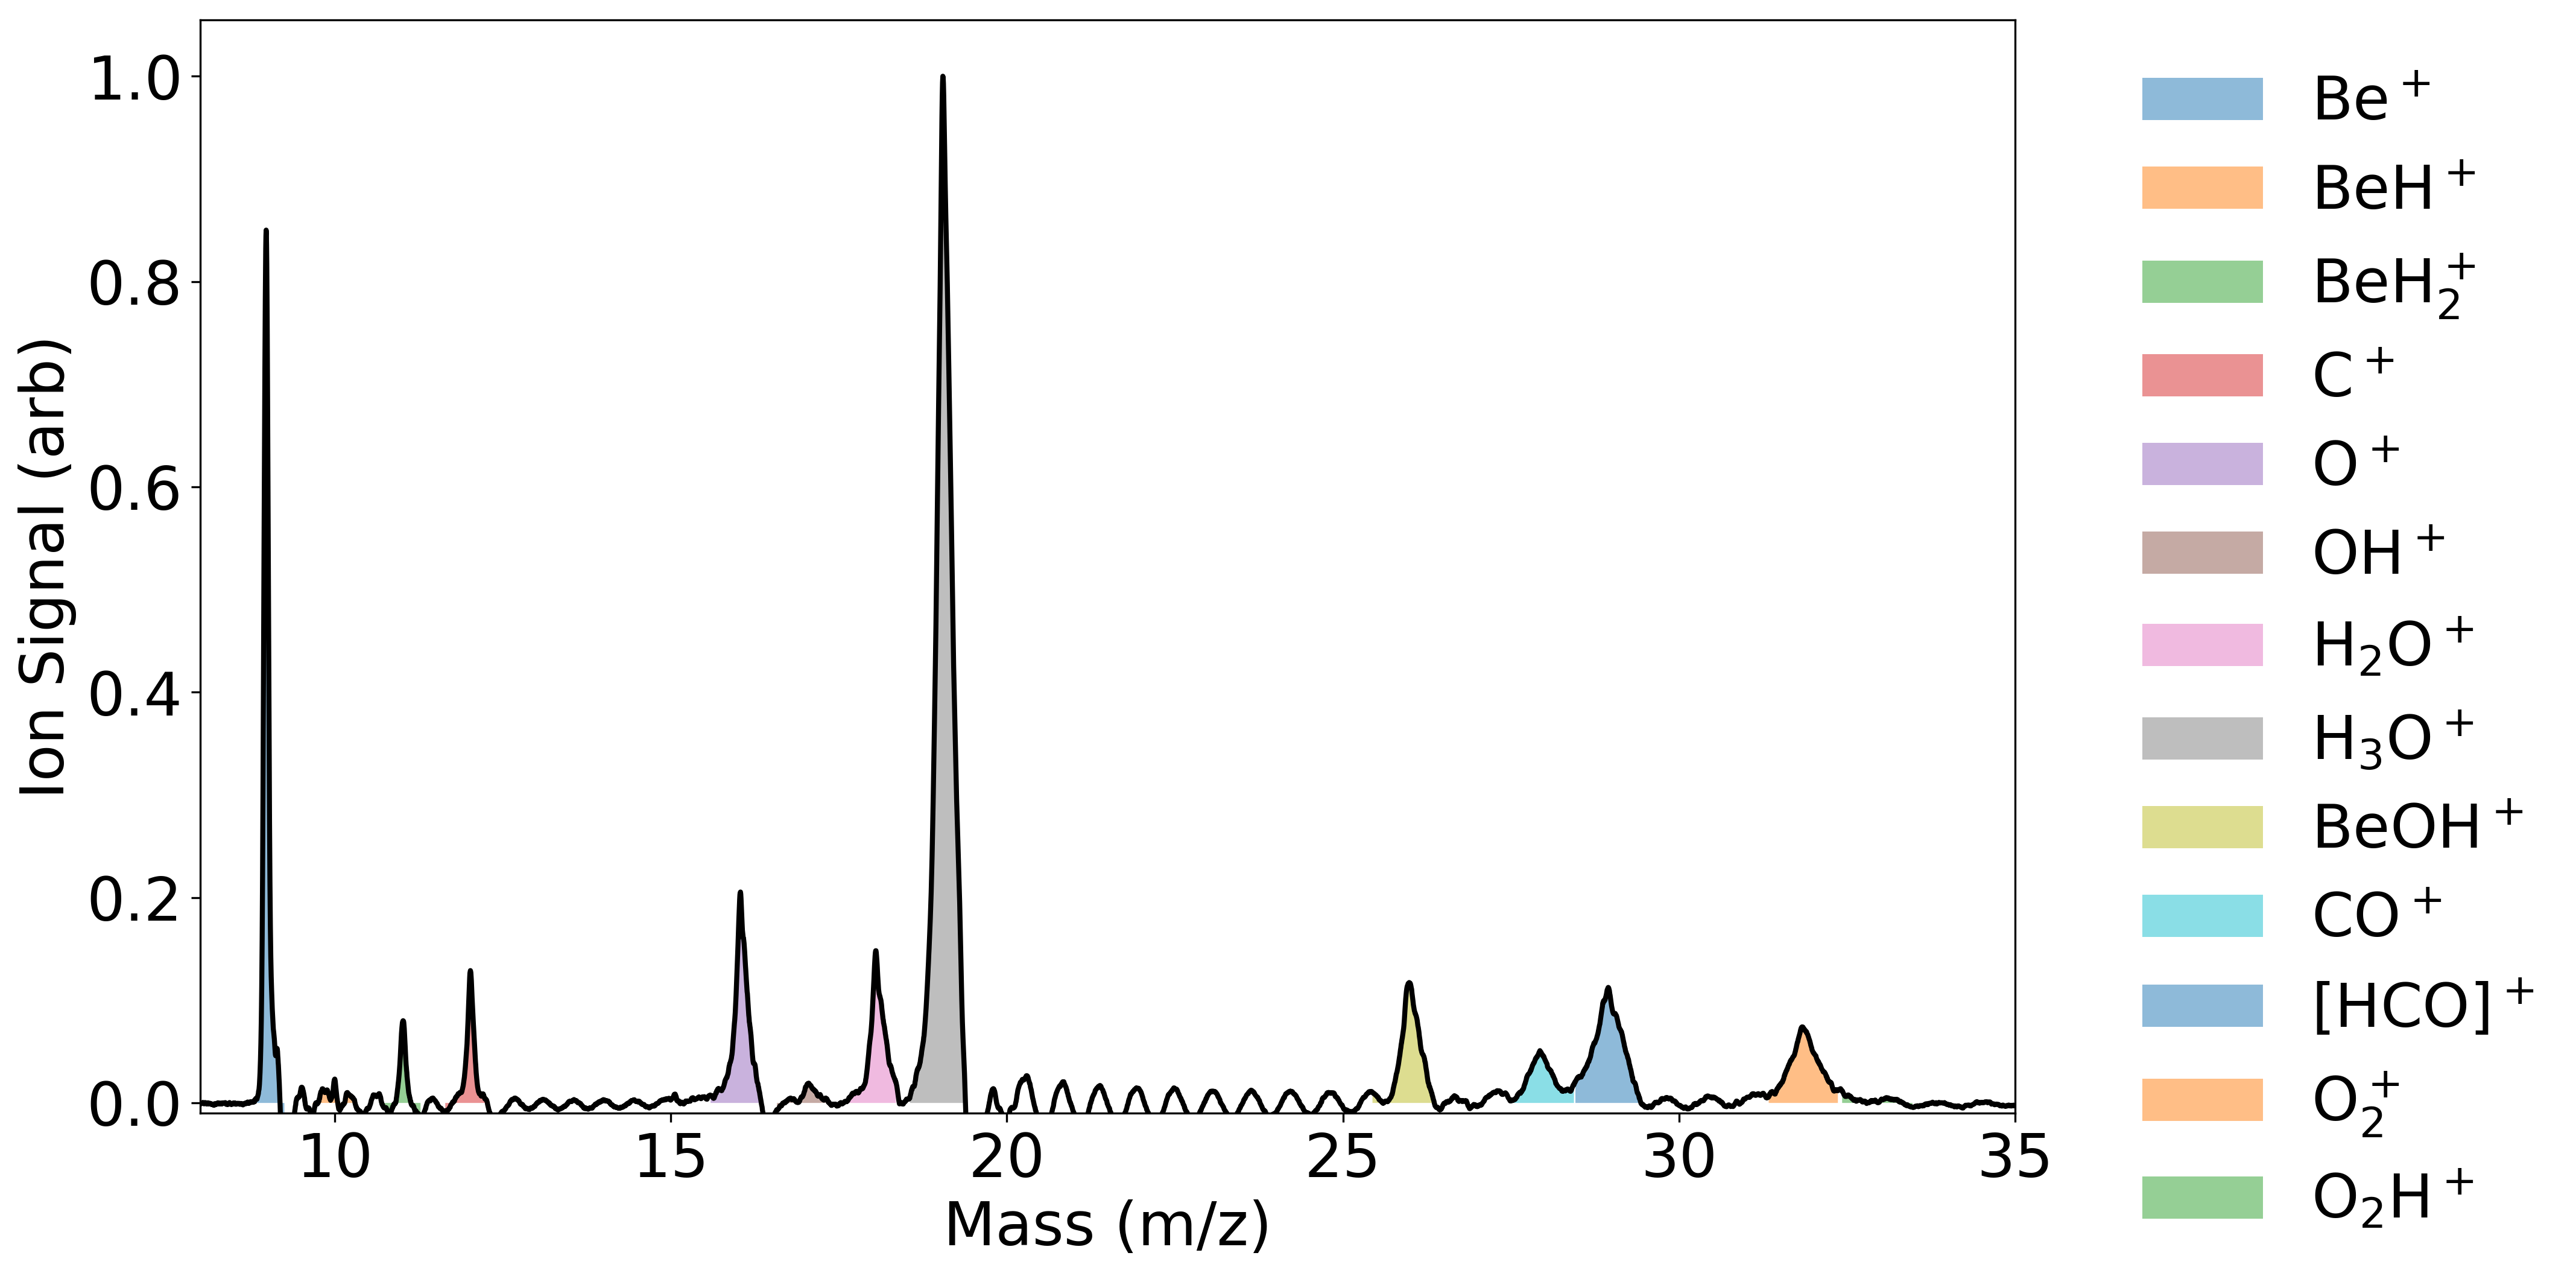
\includegraphics[width=0.8\textwidth]{images/O2_titration.png}
	\caption{Average of 10 TOF traces showing reaction products}
	\label{fig: O2 titration}
\end{figure}

There is an anomalous peaks that we do not know the origin of at $m/z=11$, which we have denoted \ce{BeH2+}. Despite this, it is clear that there is no production of \ce{O2H+}. Given a 1 s delay between the introduction of \ce{H2O} and the titration gas, the \ce{HOC+} isomer has internally relaxed to at least less than 0.2 eV. For \ce{HCO+}, there is reason to believe the the relaxation rate would be even greater, as \ce{HCO+} has a dipole moment approximately 2 times that of \ce{HOC+}.\cite{Rogers1982} With the titration gasses we use to separate the isomers, \ce{CO2} and \ce{^15N2}, the \ce{HCO+} would have to maintain an internal excited state greater than 0.48 eV and 1.05 eV, respectively, to skew the results. The lack of a proton exchange signal with \ce{O2} alleviates this concern.

%Theoretically, the probability of this 
%\begin{align*}
%	\Gamma_{\mathrm{co}} & = 2 \Gamma_1 \Gamma_2 \tau \\
%	\intertext{$\Gamma_2 \rightarrow \Gamma_1$}
%	& = 2\Gamma_1^2 \tau
%\end{align*}
%where $\Gamma_1 \approx 7 \times 10^{-3}$ s$^{-1}$, $\tau=0.3$ s, we find that $\Gamma_{\mathrm{co}} \approx 3 \times 10^{-5}$. This means, at our operating pressures, we may have 0.4\% of our signal be affected by a highly excited internal state that may cause unwanted reactions.

\section{Secondary Reactions}

As mentioned in previous sections, our ion trap continually holds the ions initially loaded, as well as the subsequent charged reaction products (within the trappable mass range). This feature is of particular importance for us, as we cannot directly read off the ratio of the isomers and will need to contend with the possibility that the two isomers will continually react with \ce{H2O} at different rates:
\begin{align}
	\ce{HCO+ + H2O & -> H3O+ + CO} \label{r: HCO+H2O->H3O} \\
	\ce{HOC+ + H2O & -> H3O+ + CO} \label{r: HOC+H2O->H3O}
\end{align}
Theoretically, the differing dipole moments of the isomers would produce different dipole-dipole interactions with \ce{H2O}. Literature shows that averaged dipole moments for \ce{HCO+} and \ce{HOC+} are 4.6 D and 2.4 D, respectively.\cite{Rogers1982} But these contribute the a induced dipole-induced dipole rate constant contribution, which is very short ranged ($1/r^6$) and do not contribute much to the overall rate constant.

We cannot deterministically measure the rate of reaction \ref{r: HOC+H2O->H3O} because there is not a way to produce only \ce{HOC+}, but we may produce only \ce{HCO+}. Considering reactions \ref{r: X+HOC->HCO} and \ref{r: X+HOC->XH}, if we let \ce{X = CO}, we find that both reactions can only yield \ce{HCO+}, allowing us to solely produce one of the isomers:
\begin{equation}
	\ce{HOC+ + CO -> HCO+ + CO} \label{r: HOC+CO->HCO}
\end{equation}
By producing only \ce{HCO+}, we directly observe reaction \ref{r: HCO+H2O->H3O}. With loaded \ce{Be+} and \ce{C+}, the trap is exposed to \ce{H2O} from the CBGB, to produce a combination of the isomers \ce{[HCO]+}, all the while, \ce{CO} is introduced via the leak valve in the differential cross region to a pressure of $\approx 4 \times 10^{-9}$ Torr as measured in the trap chamber. The constant introduction of \ce{CO} ensures full conversion of \ce{HOC+ -> HCO+} at a rate $\approx \times 10$ faster than that of reactions \ref{r: C+H2O->HCO} and \ref{r: C+H2O->HOC} ensuring we are seeing the time evolution of reaction \ref{r: HCO+H2O->H3O} as seen in Figure \ref{fig: [HCO]+H2O rate}b). A similar procedure of continuously exposing the trap to the CBGB without \ce{CO} yields a combination of the rates of reactions \ref{r: HCO+H2O->H3O} and \ref{r: HOC+H2O->H3O} seen in Figure \ref{fig: [HCO]+H2O rate}a).

The rates of reactions \ref{r: C+H2O->HCO}, \ref{r: HCO+H2O->H3O}, and a combination of reactions \ref{r: HCO+H2O->H3O}+\ref{r: HOC+H2O->H3O} are found with least-squares fitting of the solutions to differential equations found in section \ref{sec: C+H2O eqs}. Beam densities are determined for each run individually by considering the \ce{Be+ + H2O} reaction complex as outlined in Section \ref{sec: trap beam density}.

\begin{figure}[H]
	\centering
	\makebox[\textwidth][c]{
		\begin{tabular}{cc}
			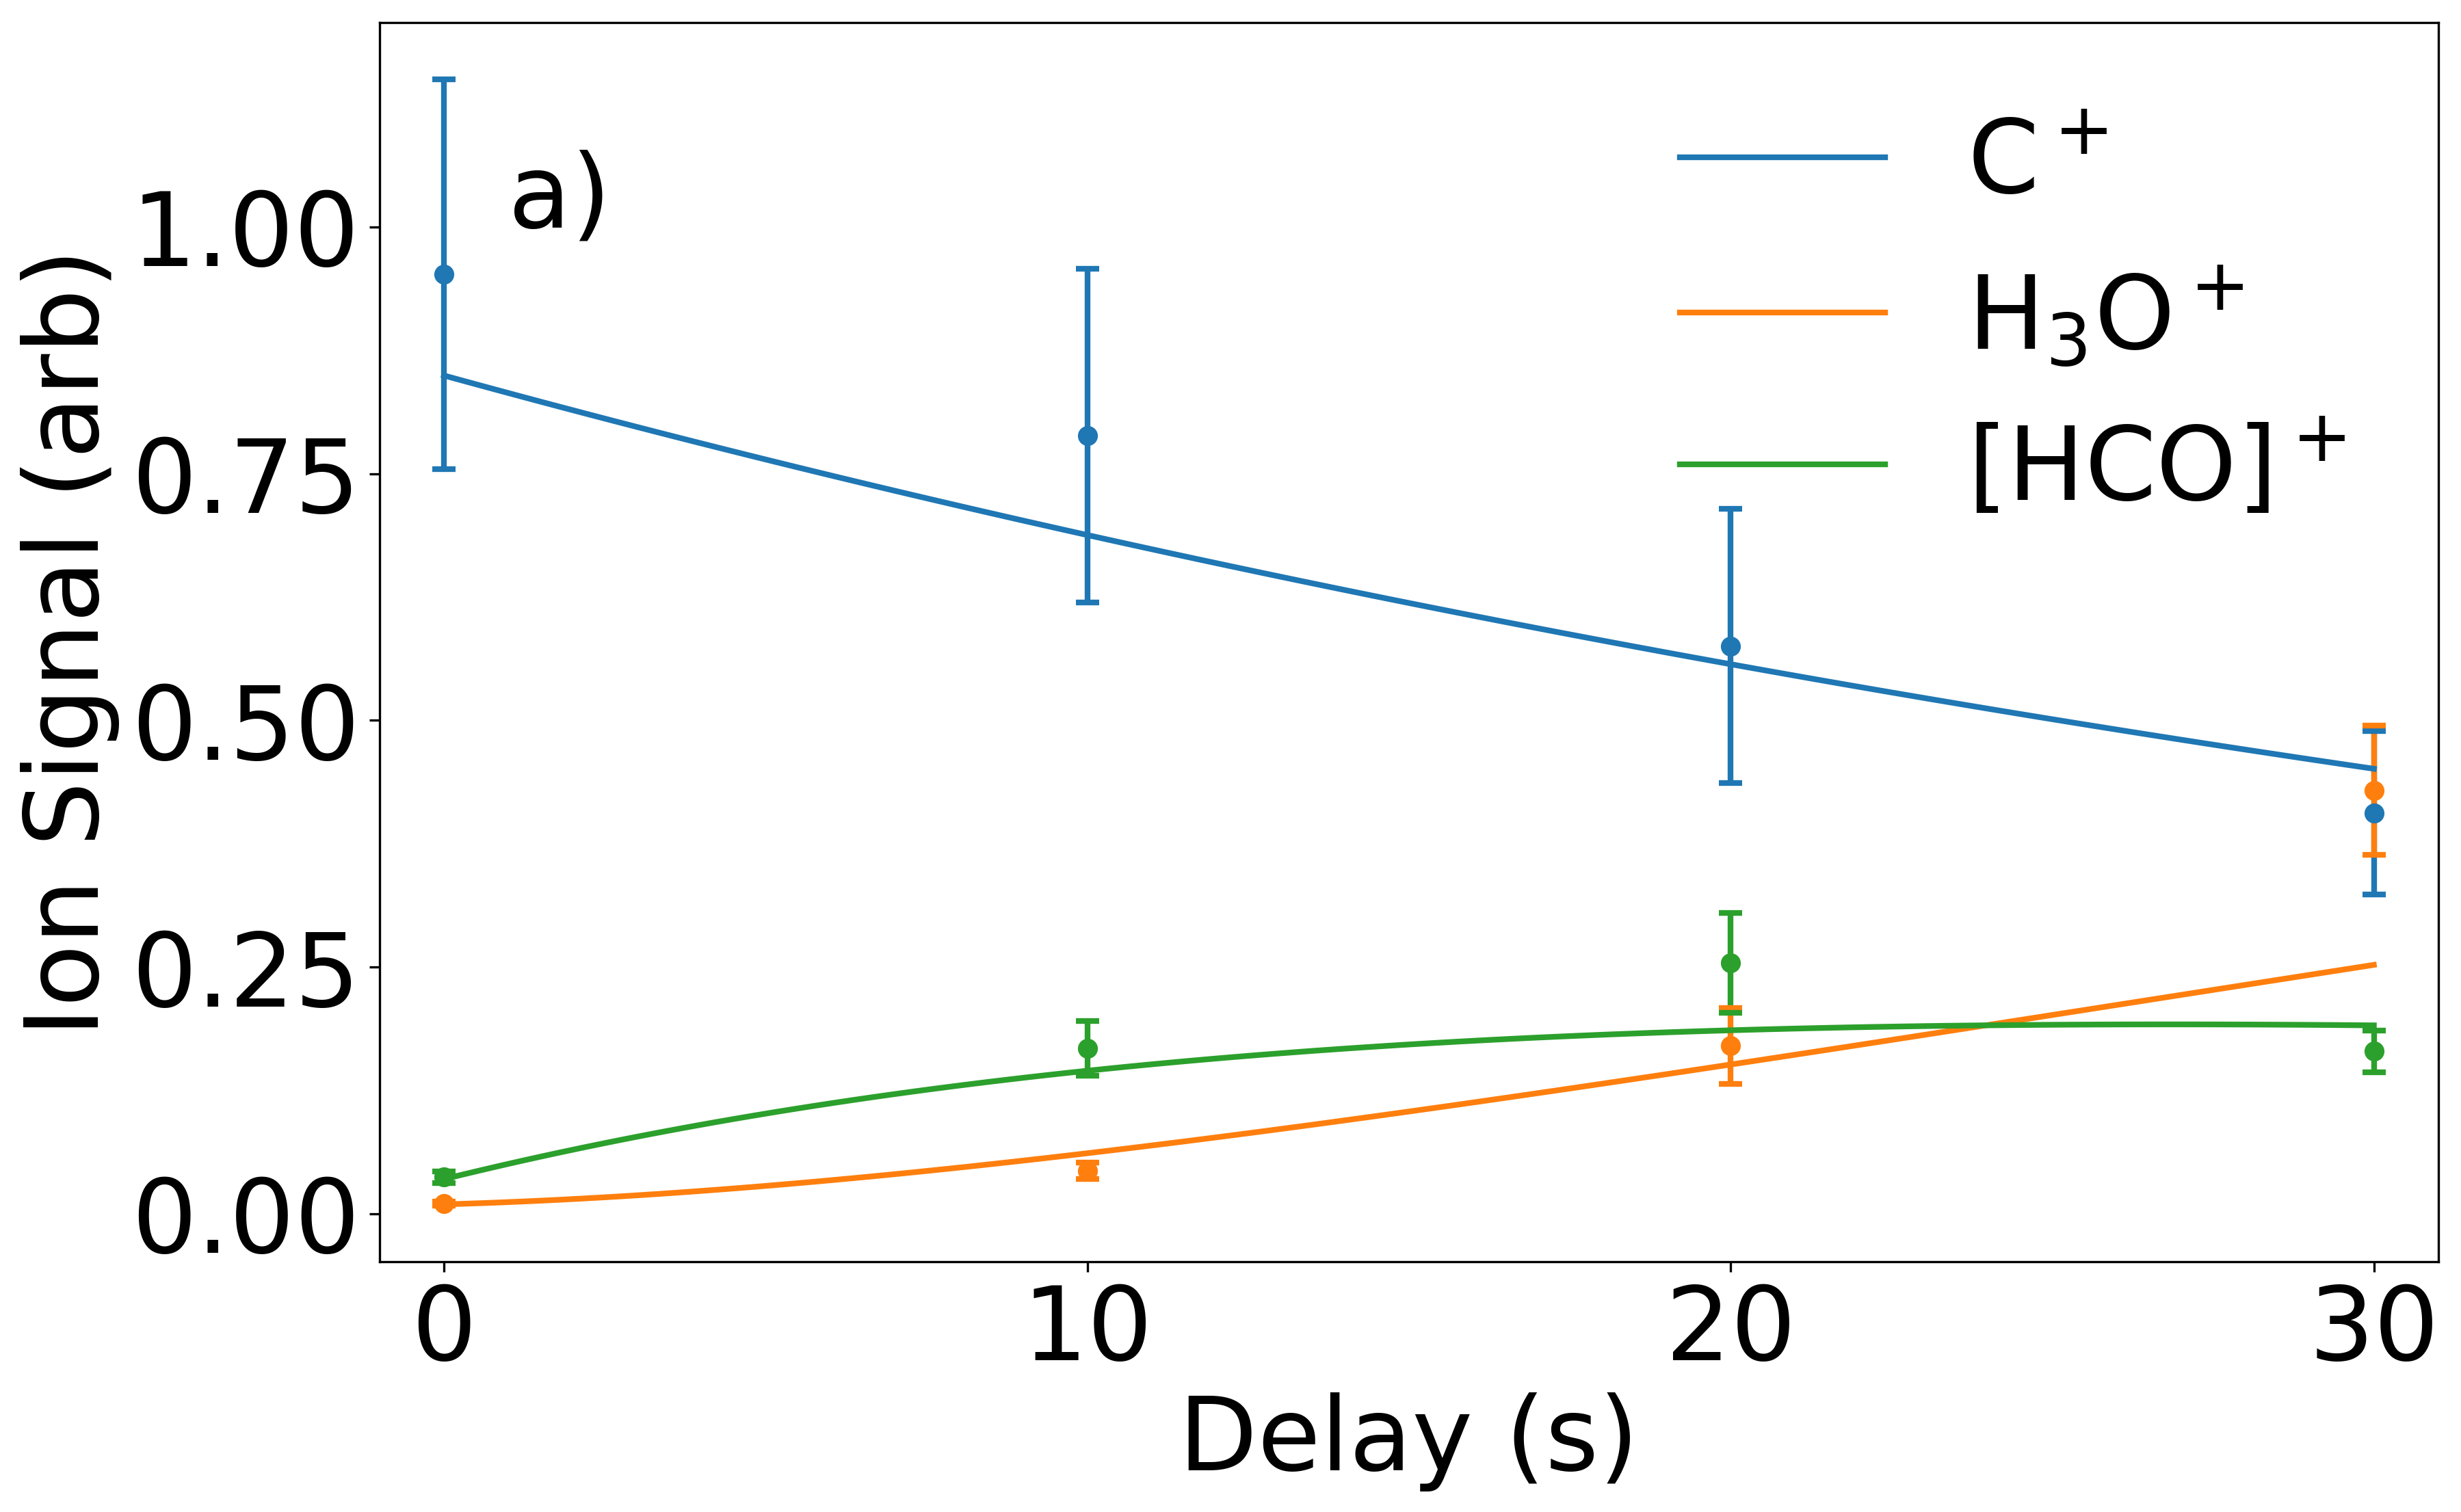
\includegraphics[width=0.5\textwidth]{images/C_H2O_beam_traces_small.png} &
			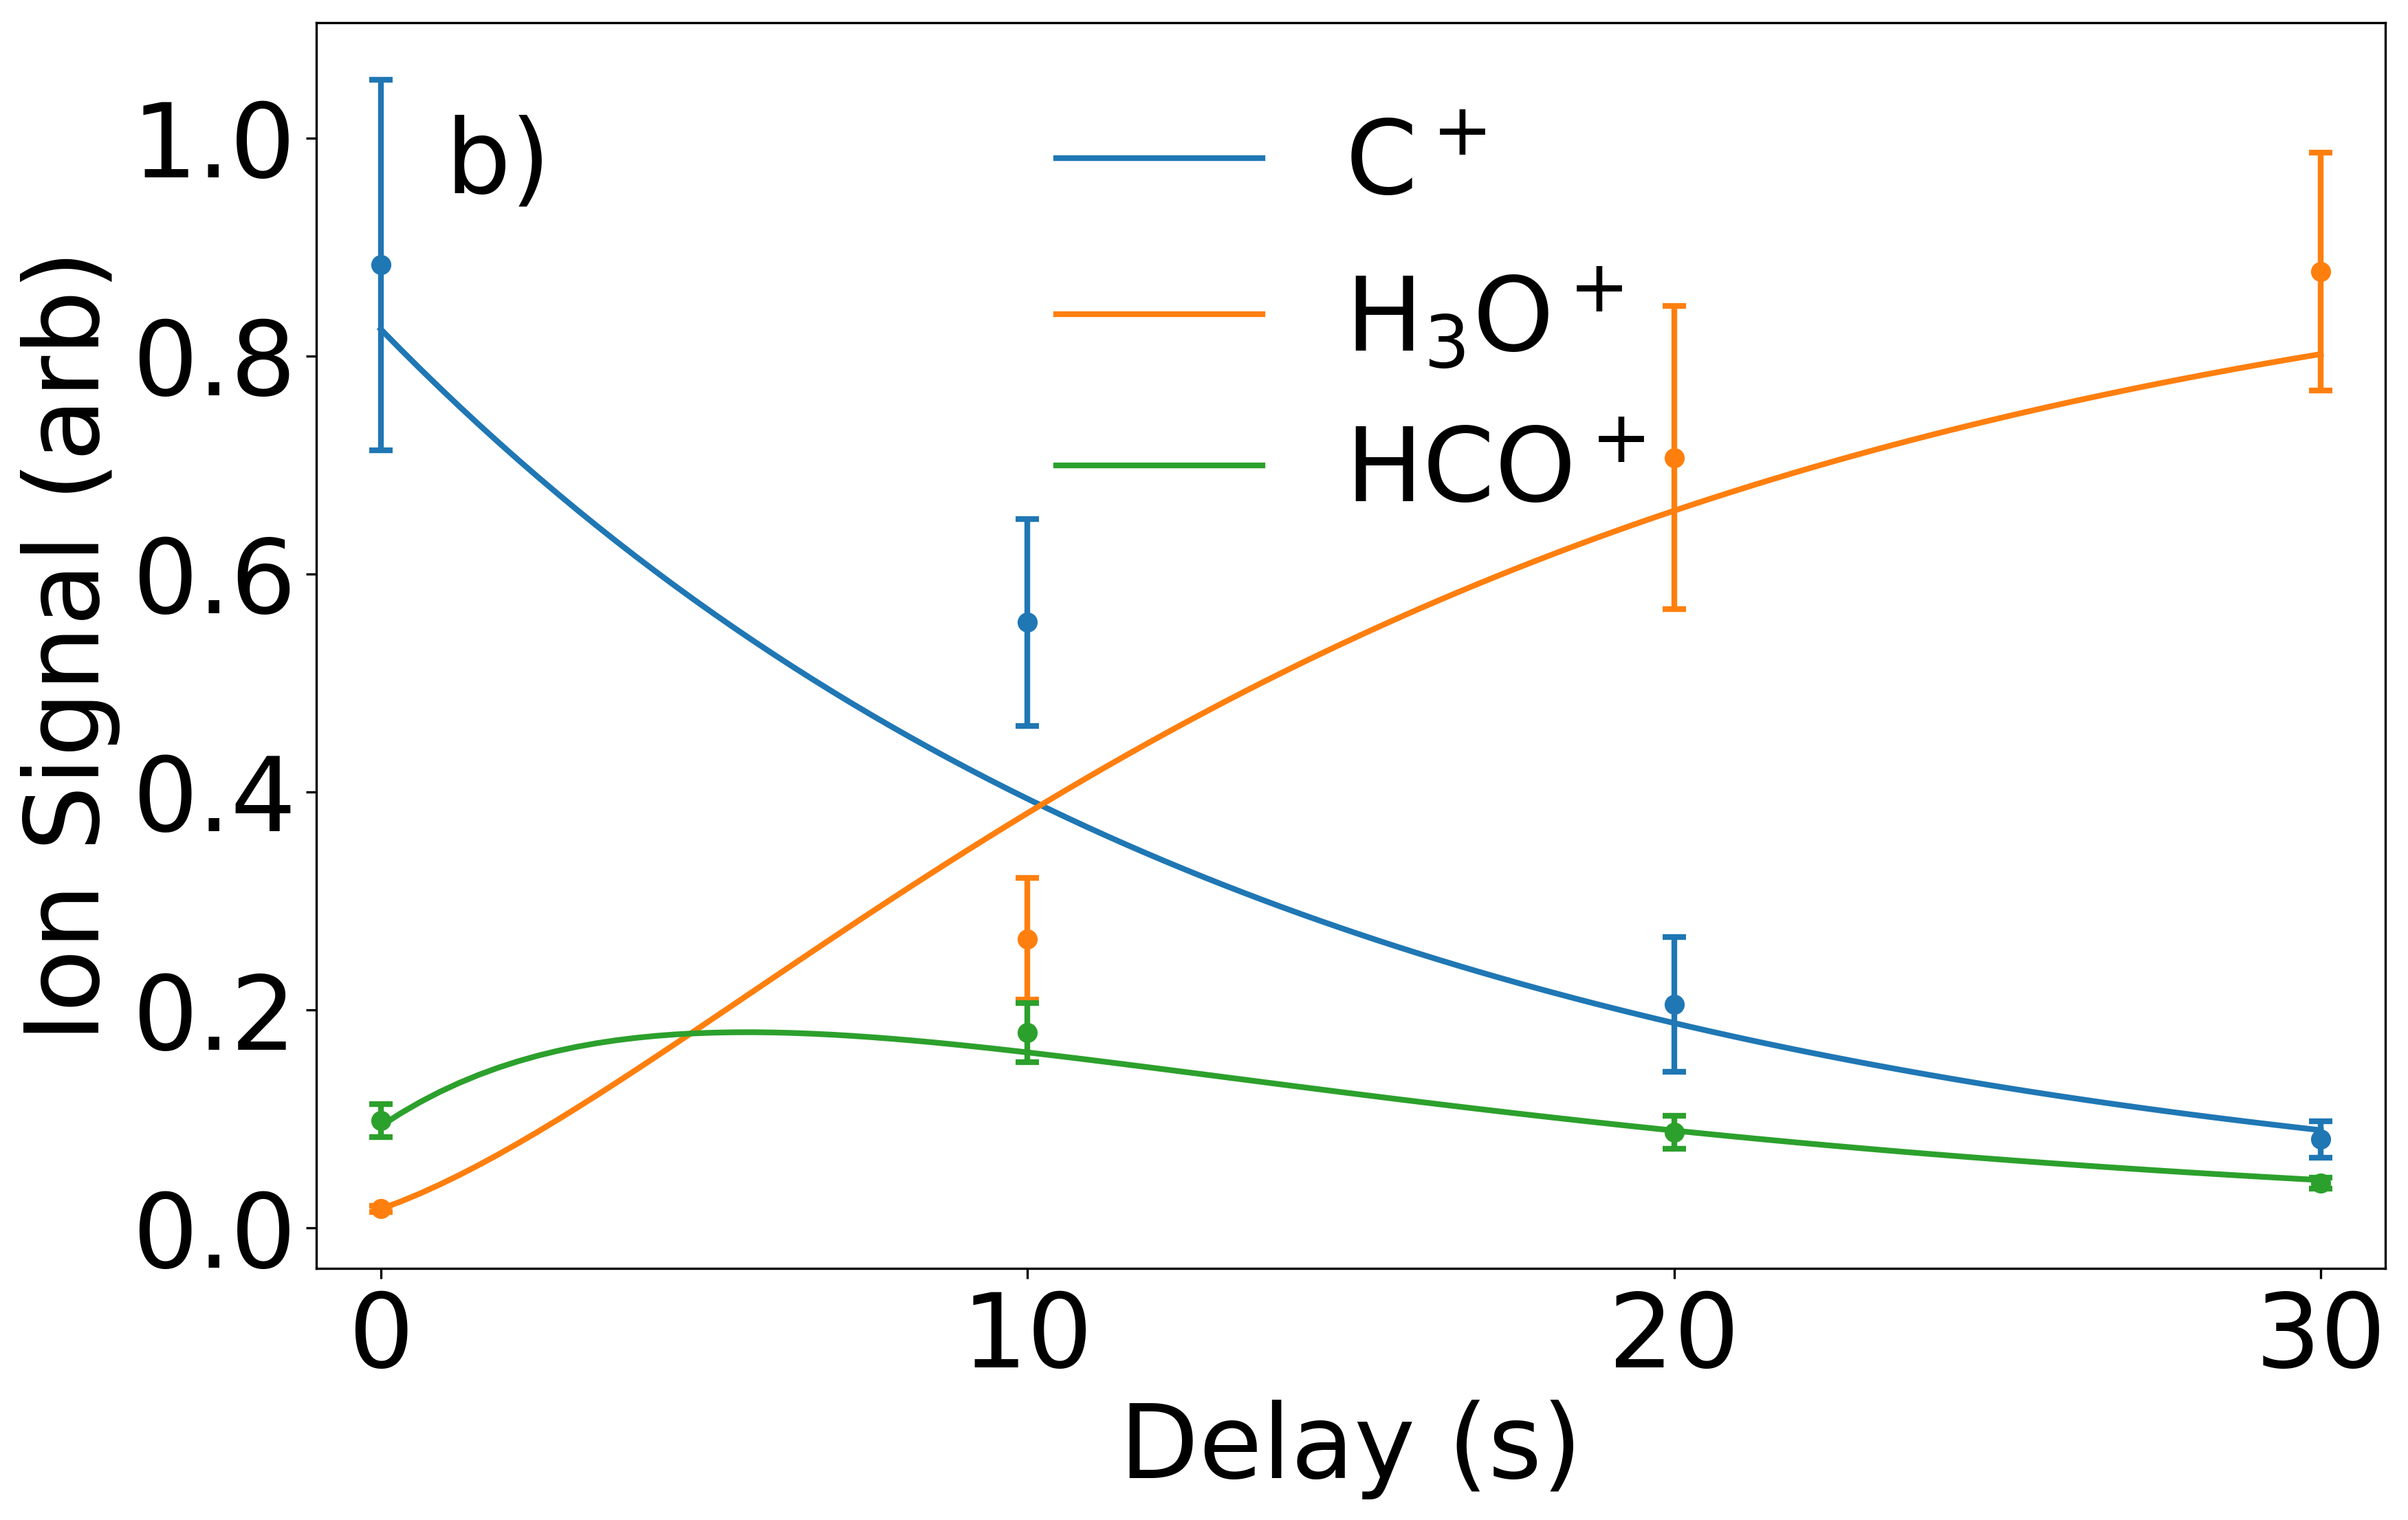
\includegraphics[width=0.5\textwidth]{images/C_H2O_CO_beam_traces_small.png}
		\end{tabular}
	}
	\caption{Time evolution of \ce{C+} and \ce{H2O} introduced via CBGB as well as subsequent reaction products. a) TOF traces without flooding of \ce{CO} where fitted rate constants are found to be $k_{\ref{r: C+H2O->HCO}}+k_{\ref{r: C+H2O->HOC}} = (7.7 \pm 0.6) \times 10^{-9}$ cm$^3$/s, and $k_{\ref{r: HCO+H2O->H3O}} = (1.7 \pm 0.2) \times 10^{-8}$ cm$^3$/s. b) TOF traces with flooding of \ce{CO} where fitted rate constants are found to be $k_{\ref{r: C+H2O->HCO}}+k_{\ref{r: C+H2O->HOC}} = (7.9 \pm 0.6) \times 10^{-9}$ cm$^3$/s, and $k_{\ref{r: [HCO]+H2O->H3O}} = (1.7 \pm 0.2) \times 10^{-8}$ cm$^3$/s.}
	\label{fig: [HCO]+H2O rate}
\end{figure}

Although we cannot make a statement about the rate of reaction \ref{r: HOC+H2O->H3O}, we see that at whatever ratio the isomers are produced, we cannot experimentally observe any meaningful deviation between the pure \ce{HCO+ + H2O} and \ce{[HCO]+ + H2O}. Thus, we find it reasonable to combine reactions \ref{r: HCO+H2O->H3O} and \ref{r: HOC+H2O->H3O} into:
\begin{equation}
	\ce{[HCO]+ + H2O -> H3O+ + CO}. \label{r: [HCO]+H2O->H3O}
\end{equation}
With this understanding, we may take the ratio of isomers at $m/z=29$ to be constant with respect to the \ce{H2O} beam exposure.

\section{Determination of Branching Ratio}

Previous literature utilized gasses such as \ce{NO}, \ce{CH4}, \ce{N2O}, and \ce{Kr} to separate the isomers.\cite{Love1987} Of those \ce{Kr}, and \ce{Xe} are inert and would not react with any other ions in our trap, but are too heavy to reliably hold after a reaction. Of the others, \ce{NO} is caustic and will ruin the vacuum chamber if introduced, and thus was avoided. Attempts were make with \ce{N2O} and well as \ce{CH4}, but both had their own unique complications. \ce{N2O} rapidly reacts with \ce{Be+} and made reliable TOF traces unattainable due to the loss of the coolant ion. \ce{CH4} readily reacted with most of the ions in the trap to produce a multitude of mass peaks, greatly complicating the analysis with secondary, tertiary, and higher order reactions. In this section, I describe the methods and results using \ce{CO2} and \ce{^15N2} gasses to separate the isomer mass signatures.

\subsection{\ce{CO2} Titration}

From table \ref{tab: affinities}, we see that \ce{CO2} is a viable option to titrate the reaction products. The possible reactions of \ce{CO2} with \ce{Be+} are unknown in literature, but found to be non-reactive in both ground and excited states, while \ce{C+} readily reacts
\begin{align}
	\ce{Be+ + CO2 & -> no reaction} \nonumber \\
	\ce{C+ + CO2 & -> CO+ + CO} \label{r: C+CO2->CO} \\
	\ce{& -> CO2+ + C} \label{r: C+CO2->CO2} \\
	\ce{CO+ + CO2 & -> CO2+ + CO}. \label{r: CO+CO2->CO2}
\end{align}
Being non-reactive with \ce{Be+} while having a product mass that is still within our trappable range makes \ce{CO2} an attractive option. Its reactivity with \ce{C+} is both a detriment, as well as a useful tool. If the \ce{C+} has been depleted via reactions \ref{r: C+CO2->CO} and \ref{r: C+CO2->CO2}, all the \ce{HOC+} should also have undergone reaction \ref{r: X+HOC->XH}.

%Testing the purity of the \ce{CO2}, I introduce the \ce{CO2} into the ion chamber with the RGA.
%
%\begin{figure}[H]
%	\centering
%	\includegraphics[width=0.7\textwidth]{images/C_CO2_rga.png}
%	\caption{\label{fig: cco2 rga} RGA showing purity of \ce{CO2} introduced into chamber. Ratios of \ce{CO2} peaks at $m/z = 12, 16, 28$, and $44$ in agreement with table \ref{t: cco2 fractionation}, with no conclusive evidence of contamination by any other gas.}
%\end{figure}

%\begin{table}[H]
%	\centering
%	\label{t: cco2 fractionation}
%	\begin{tabular}{|l|l| }
%	\hline
%	m/z & Fraction \\
%	\hline
%	44 & 0.85 \\
%	28 & 0.05 \\
%	16 & 0.05 \\
%	12 & 0.012 \\
%	\hline
%	\end{tabular}
%	\caption{RGA fractionation of \ce{CO2} as given by http://ytionline.com/technical-information/rga-spectra-data-fragmentation-factor/}
%\end{table}

\subsubsection{\ce{C+ + CO2}}
By ablating both \ce{C+} and \ce{Be+} into the trap and introducing \ce{CO2} via the leak valve, we find the expected reactions \ref{r: C+CO2->CO}, \ref{r: C+CO2->CO2}, and \ref{r: CO+CO2->CO2} as well as unexpected peaks appearing at $m/z=15, 29$, and $45$.

\begin{figure}
	\label{fig: C+CO2 TOF}
	\centering
	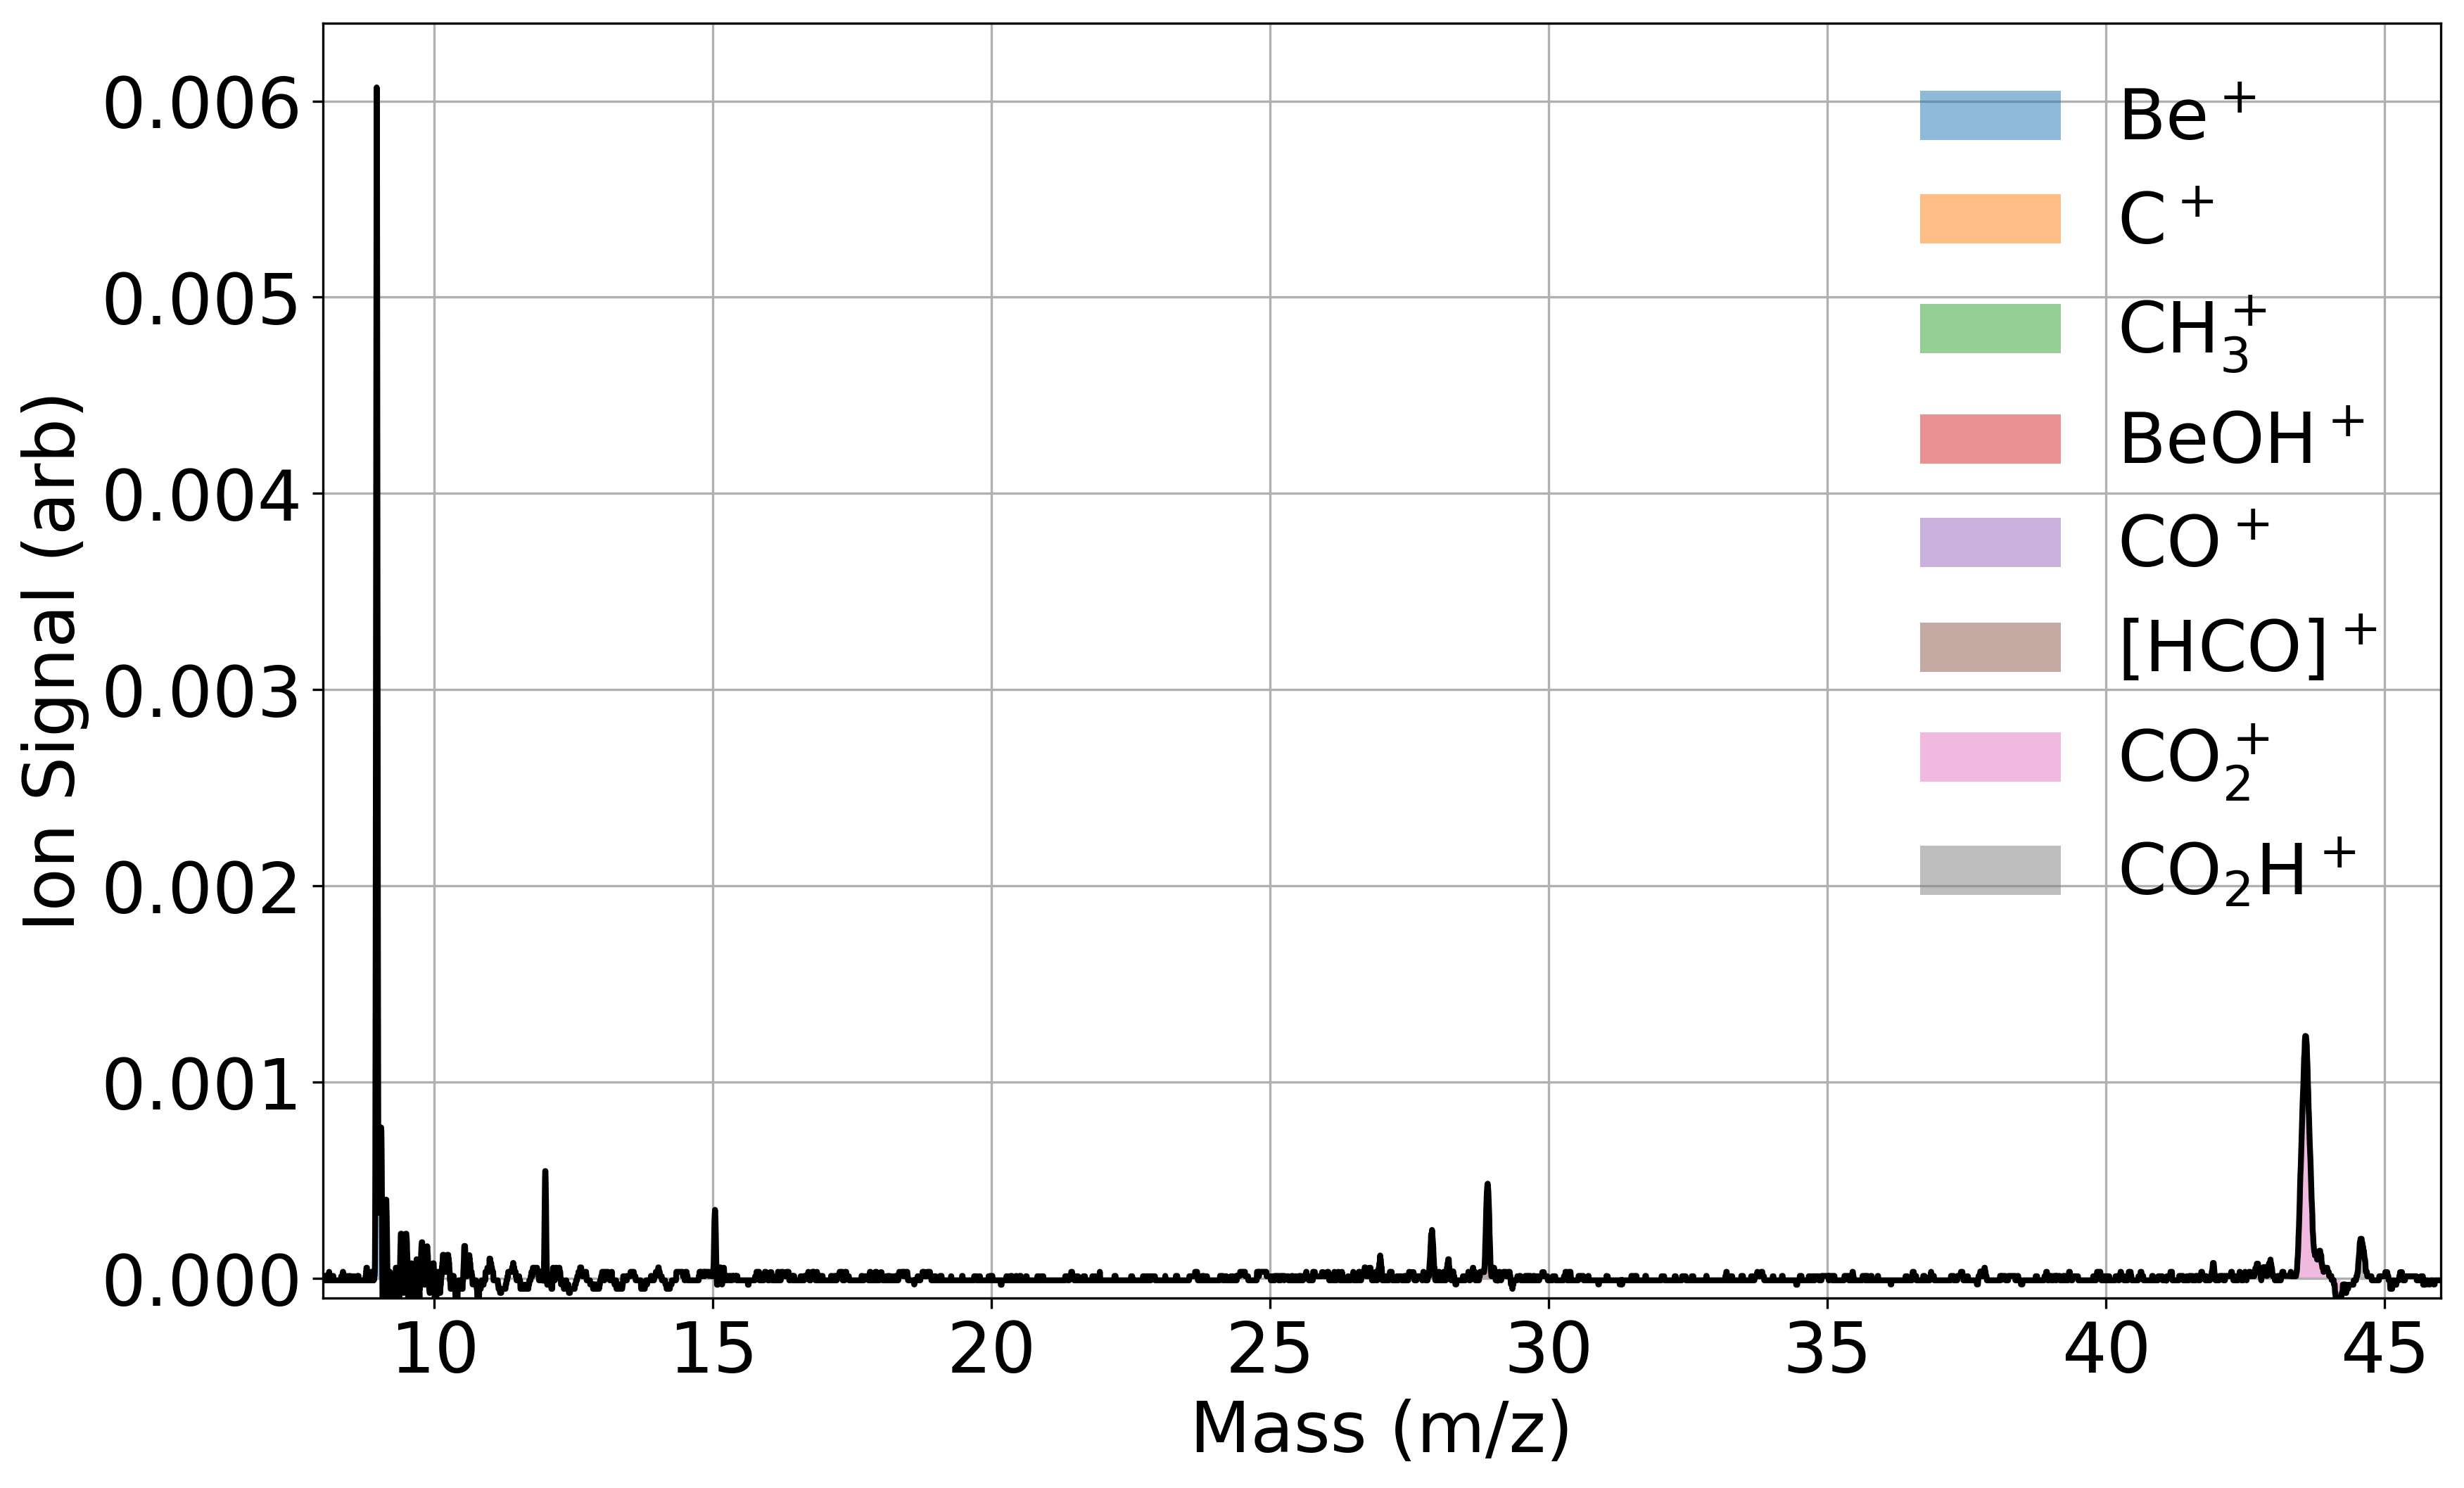
\includegraphics[width=0.8\textwidth]{images/C_CO2_TOF.png}
	\caption{TOF trace of laser-cooled \ce{Be+} and \ce{C+} reacting with $\approx 1 \times 10^{-8}$ Torr \ce{CO2} introduced via leak valve for 40 seconds.}
\end{figure}

\begin{figure}
	\label{fig: C+CO2 traces}
	\centering
	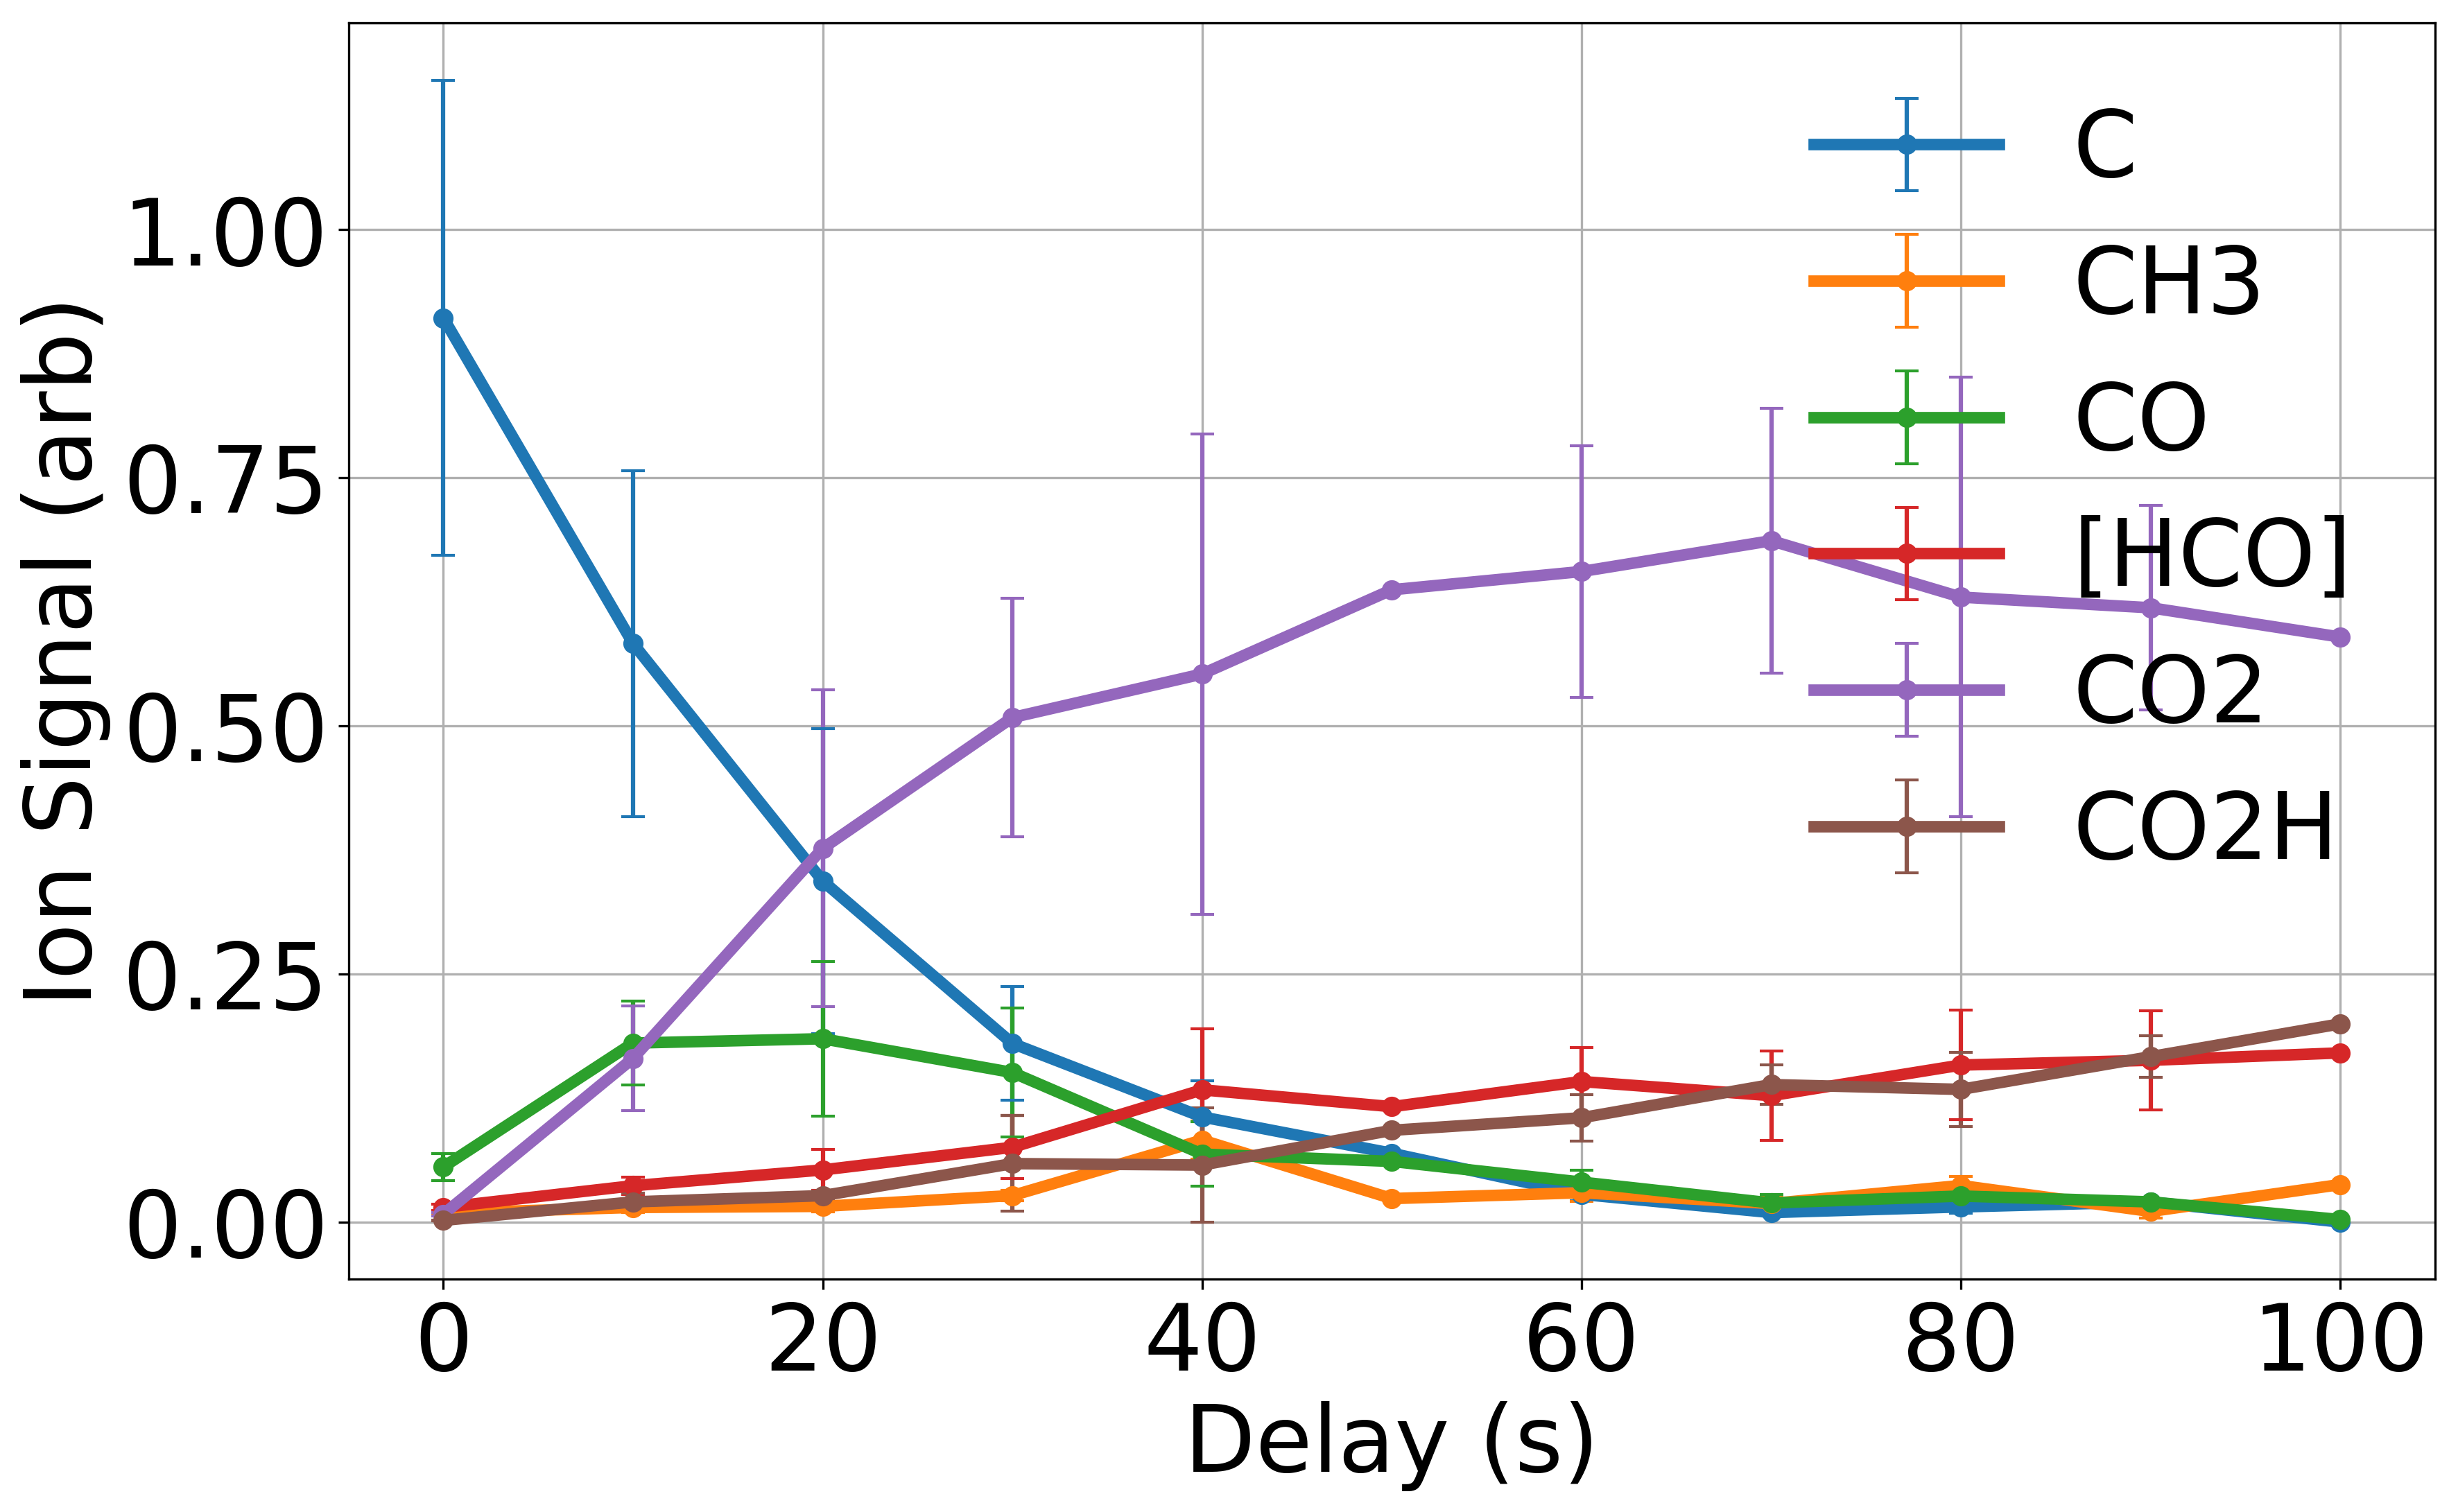
\includegraphics[width=0.8\textwidth]{images/C_CO2_traces.png}
	\caption{Integrated ion signal of individual TOF traces normalized by total ion signal excluding \ce{Be+} at various \ce{CO2} exposure times.}
\end{figure}

Labels in Figures \ref{fig: C+CO2 TOF} and \ref{fig: C+CO2 traces} are of predicted chemicals coinciding with the masses. These peaks suggest contamination with stray \ce{H2O} in the leak valve, but the lack of a $m/z=26$ peak, coinciding with \ce{BeOH+}, suggests this is not due to \ce{H2O}. We should also expect to see an abundance of \ce{H3O+} due to reactions between the alleged \ce{[HCO]+} and \ce{CO2H+}, which we also do not see. Furthermore, the inclusion of \ce{H2O} does not explain the appearance of $m/z=15$.
\begin{align}
	\ce{CO+ + H2O & -> H2O+ + CO} \\
	\ce{CO2+ + H2O & -> CO2H+ + OH} \label{r: CO2+H2O->CO2H} \\
	\ce{CO2H+ + H2O & -> H3O+ + CO2}
\end{align}
I still doubt that the 29 mass is due to \ce{C+} directly reacting with \ce{H2O} because the traces clearly show it increasing despite the depletion of \ce{C+}, indicating it is a second order reaction. It wouldn't be \ce{H2} either, because we would see \ce{BeH+} in the trap, as well as many other peaks associated with \ce{C+ + H2} including 14, 16, and 17.

\subsubsection{\ce{Be+ + C+ + H2O} with \ce{CO2}}
Water is introduced into the chamber via the CBGB with the cell held at a temperature of 20K. After $(10 \pm 1)$ seconds of exposure, the gate valve is closed and \ce{CO2} is leaked in to react away the formyl isomers such that $\approx 99\%$ are reacted away (determined by the disappearance of \ce{C+}).

\begin{figure}[H]
	\centering
	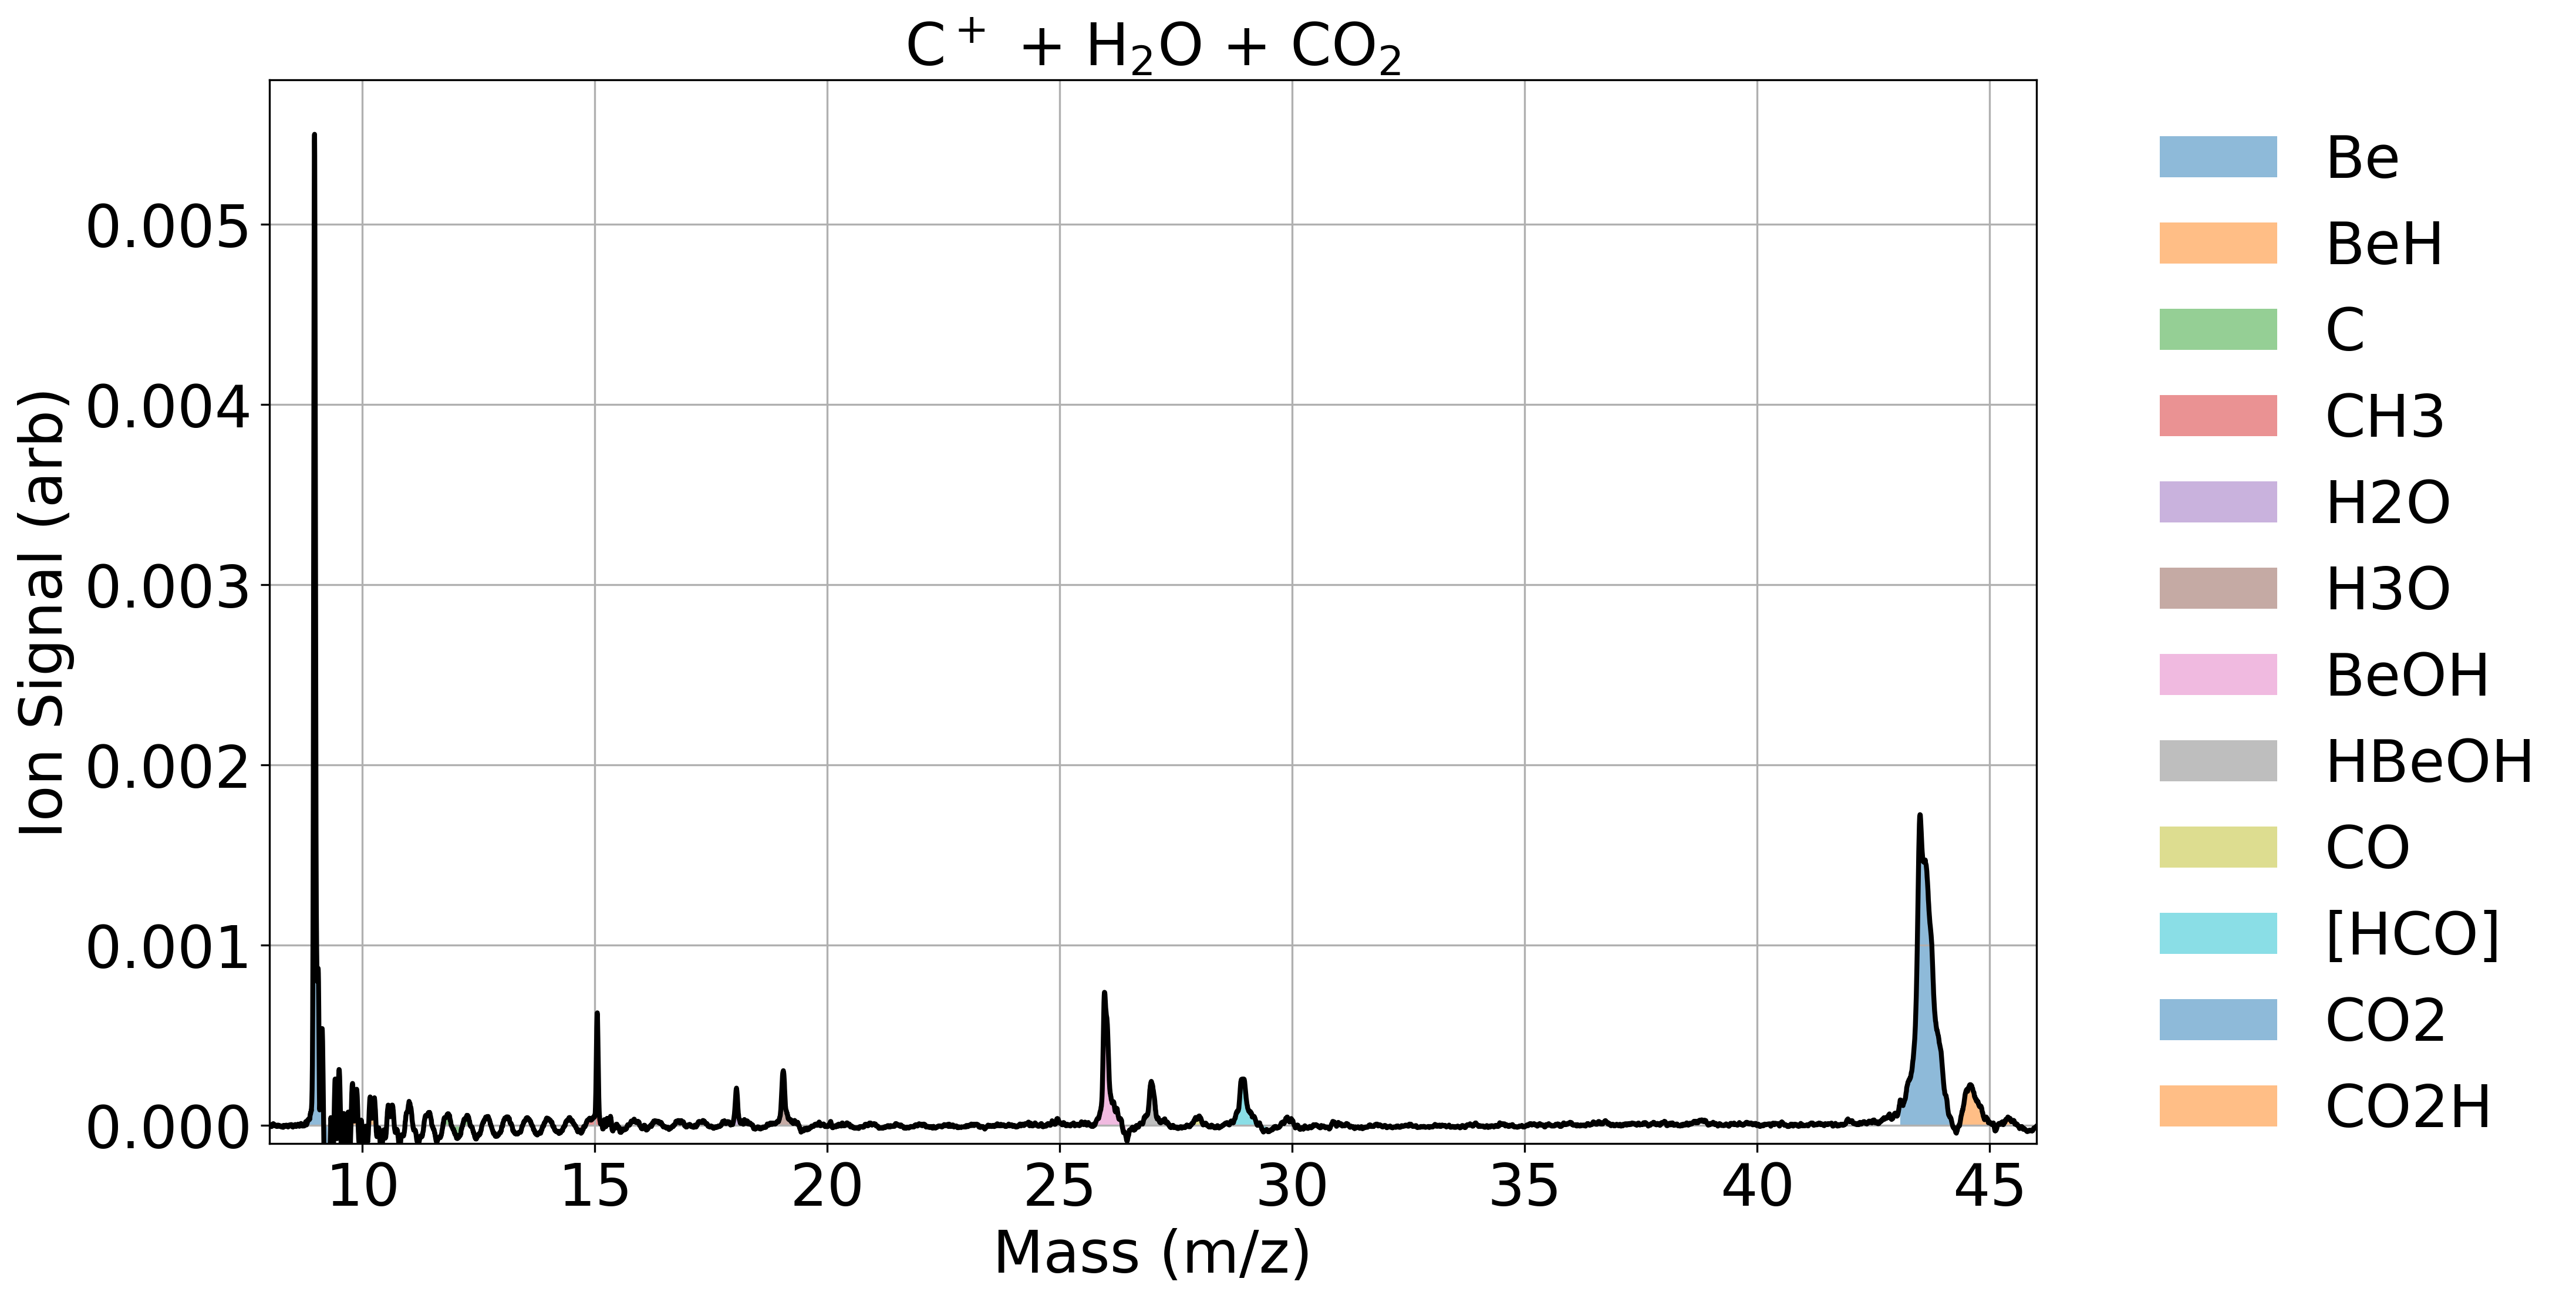
\includegraphics[width=0.9\textwidth]{images/C_H2O_CO2_titration_TOF.png}
	\caption{\ce{C+} and \ce{Be+} loaded into the trap is reacted with \ce{H2O} introduced from the beam. The gate valve is closed after 10 seconds and \ce{CO2} is introduced via leak valve so that the \ce{HOC+} is titrated into \ce{CO2H+}.}
\end{figure}

Knowing the anomalous peaks in the previous tests, the peaks of interest are not exclusively the branching ratio between the formyl isomers, where we define $\gamma$ as the fraction of products that produce \ce{HOC+}. By taking the solutions to the differential equations for the \ce{C+ + H2O} reaction network in Section \ref{sec: C+H2O eqs}, we define the ratio of the formyl isomers and remaining \ce{C+}.

\begin{equation}
	\alpha(t) \equiv \frac{\ce{[HCO](t)}}{\ce{[HCO](t) + C(t)}}
\end{equation}

In the data taken, we introduced the water in the beam for approximately 10s, the fraction of \ce{C+} that has turned into \ce{[HCO]+} is thus $\alpha = 0.37 \pm 0.02$. Considering that after titration with \ce{CO2}, the fraction of the remaining 63\% of \ce{C+} has turned into equal amounts of $m/z=29, 45$ defined as $\beta = 0.17 \pm 0.02$.
\begin{align*}
	N_C(0) & = N_0 \\
	N_C(\tau_1) & = (1-\alpha(\tau_1))N_0 \\
	N_{29}(\tau_1) & = \alpha(\tau_1) N_0
\end{align*}
Where $N_C(t)$ is the amount of \ce{C+} is in the trap after being exposed to either the water beam or \ce{CO2} for time $t$. $\tau_1$ is the amount of time where the ions are exposed to the water beam, where $\alpha$ is the proportion of \ce{C+} that is converted to $m/z=29$, which in our case is 0.37. We then introduce the \ce{CO2} into the system and yield:
\begin{align*}
	N_C(\tau_1 + \tau_2) & = 0 \\
	N_{29}(\tau_1 + \tau_2) & = N_{29}(\tau_1)(1-\gamma) + N_C(\tau_1)\beta \\
	& = N_0(\alpha(1-\gamma)+\beta(1-\alpha)) \\
	N_{45}(\tau_1 + \tau_2) & = N_{29}(\tau_1)\gamma + N_C(\tau_1)\beta \\
	& = N_0(\alpha \gamma+\beta(1-\alpha))
\end{align*}
The directly measured ratio $\eta \equiv \frac{\ce{CO2H+}}{\ce{CO2H+} + \ce{HCO+}} = 0.55 \pm 0.02$, is equated to the combination of the possible sources of competing mass peaks:
\begin{align}
	\eta = 0.55 & = \frac{N_{45}(\tau_1 + \tau_2)}{N_{29}(\tau_1 + \tau_2) + N_{45}(\tau_1 + \tau_2)}
\end{align}
To find the branching ratio of the \ce{HOC+} channel, we solve for $\gamma$:
\begin{align}
	\eta & = \frac{\beta - \alpha \beta + \alpha \gamma}{\alpha + 2\beta - 2\alpha\beta} \nonumber \\
	\gamma & = \frac{1}{\alpha} (\alpha \eta + \beta(\alpha + 2\eta - 2\alpha \eta - 1)) \label{e: gamma branching ratio}
\end{align}
Using equation \ref{e: gamma branching ratio}, we find at the true branching ratio is scaled from $0.55 \pm 0.03$ to $0.58 \pm 0.05$. The error bars are fairly large on this measurement due to the unknown species contributing to our direct ratio measurement.

\subsection{\ce{^{15}N2} Titration}

Normally \ce{N2} would not be a good choice, due to the fact that \ce{N2H+} has the same mass as the formyl isomers at $m/z=29$, but we may instead introduce \ce{^{15}N2} to produce a new peak at $m/z=31$. We do not expect and do not see any reaction between the initially loaded ions of \ce{Be+} and \ce{C+} making this the ideal candidate for titration. But according to \cref{tab: affinities}, we should still have a separation of the isomers, thus:
\begin{align}
\ce{Be+ + ^15N2 & -> no reaction} \nonumber \\
\ce{C+ + ^15N2 & -> no reaction} \nonumber \\
\ce{HCO+ + ^15N2 & -> no reaction} \label{r: HCO+N2->NA} \\
\ce{HOC+ + ^15N2 & -> ^15N2H+ + CO} \label{r: HOC+N2->N2H}
\end{align}
To verify reaction \ref{r: HOC+CO->HCO}, trapped \ce{Be+} and \ce{C+} ions are exposed to the water from the CBGB at a density of $4.3 \times 10^6$ cm$^{-3}$ while simultaneously flooded with $\approx 3 \times 10^7$ cm$^{-3}$ of \ce{CO} from the leak valve connected to the differential pumping region such that $k_{\ref{r: HOC+CO->HCO}} \gg k_{\ref{r: C+H2O->HCO}, \ref{r: C+H2O->HOC}}$. After $\sim$10 s, the gate valve between the differential pumping and experimental ion chamber regions is manually closed, after which, $10^9$ cm$^{-3}$ of \ce{^15N2} is introduced for $\sim$10 s. A TOF trace for this procedure is seen in figure \ref{fig: CO N2 TOF}, showing clear lack of \ce{^15N2H+}.

\begin{figure}[H]
	\centering
	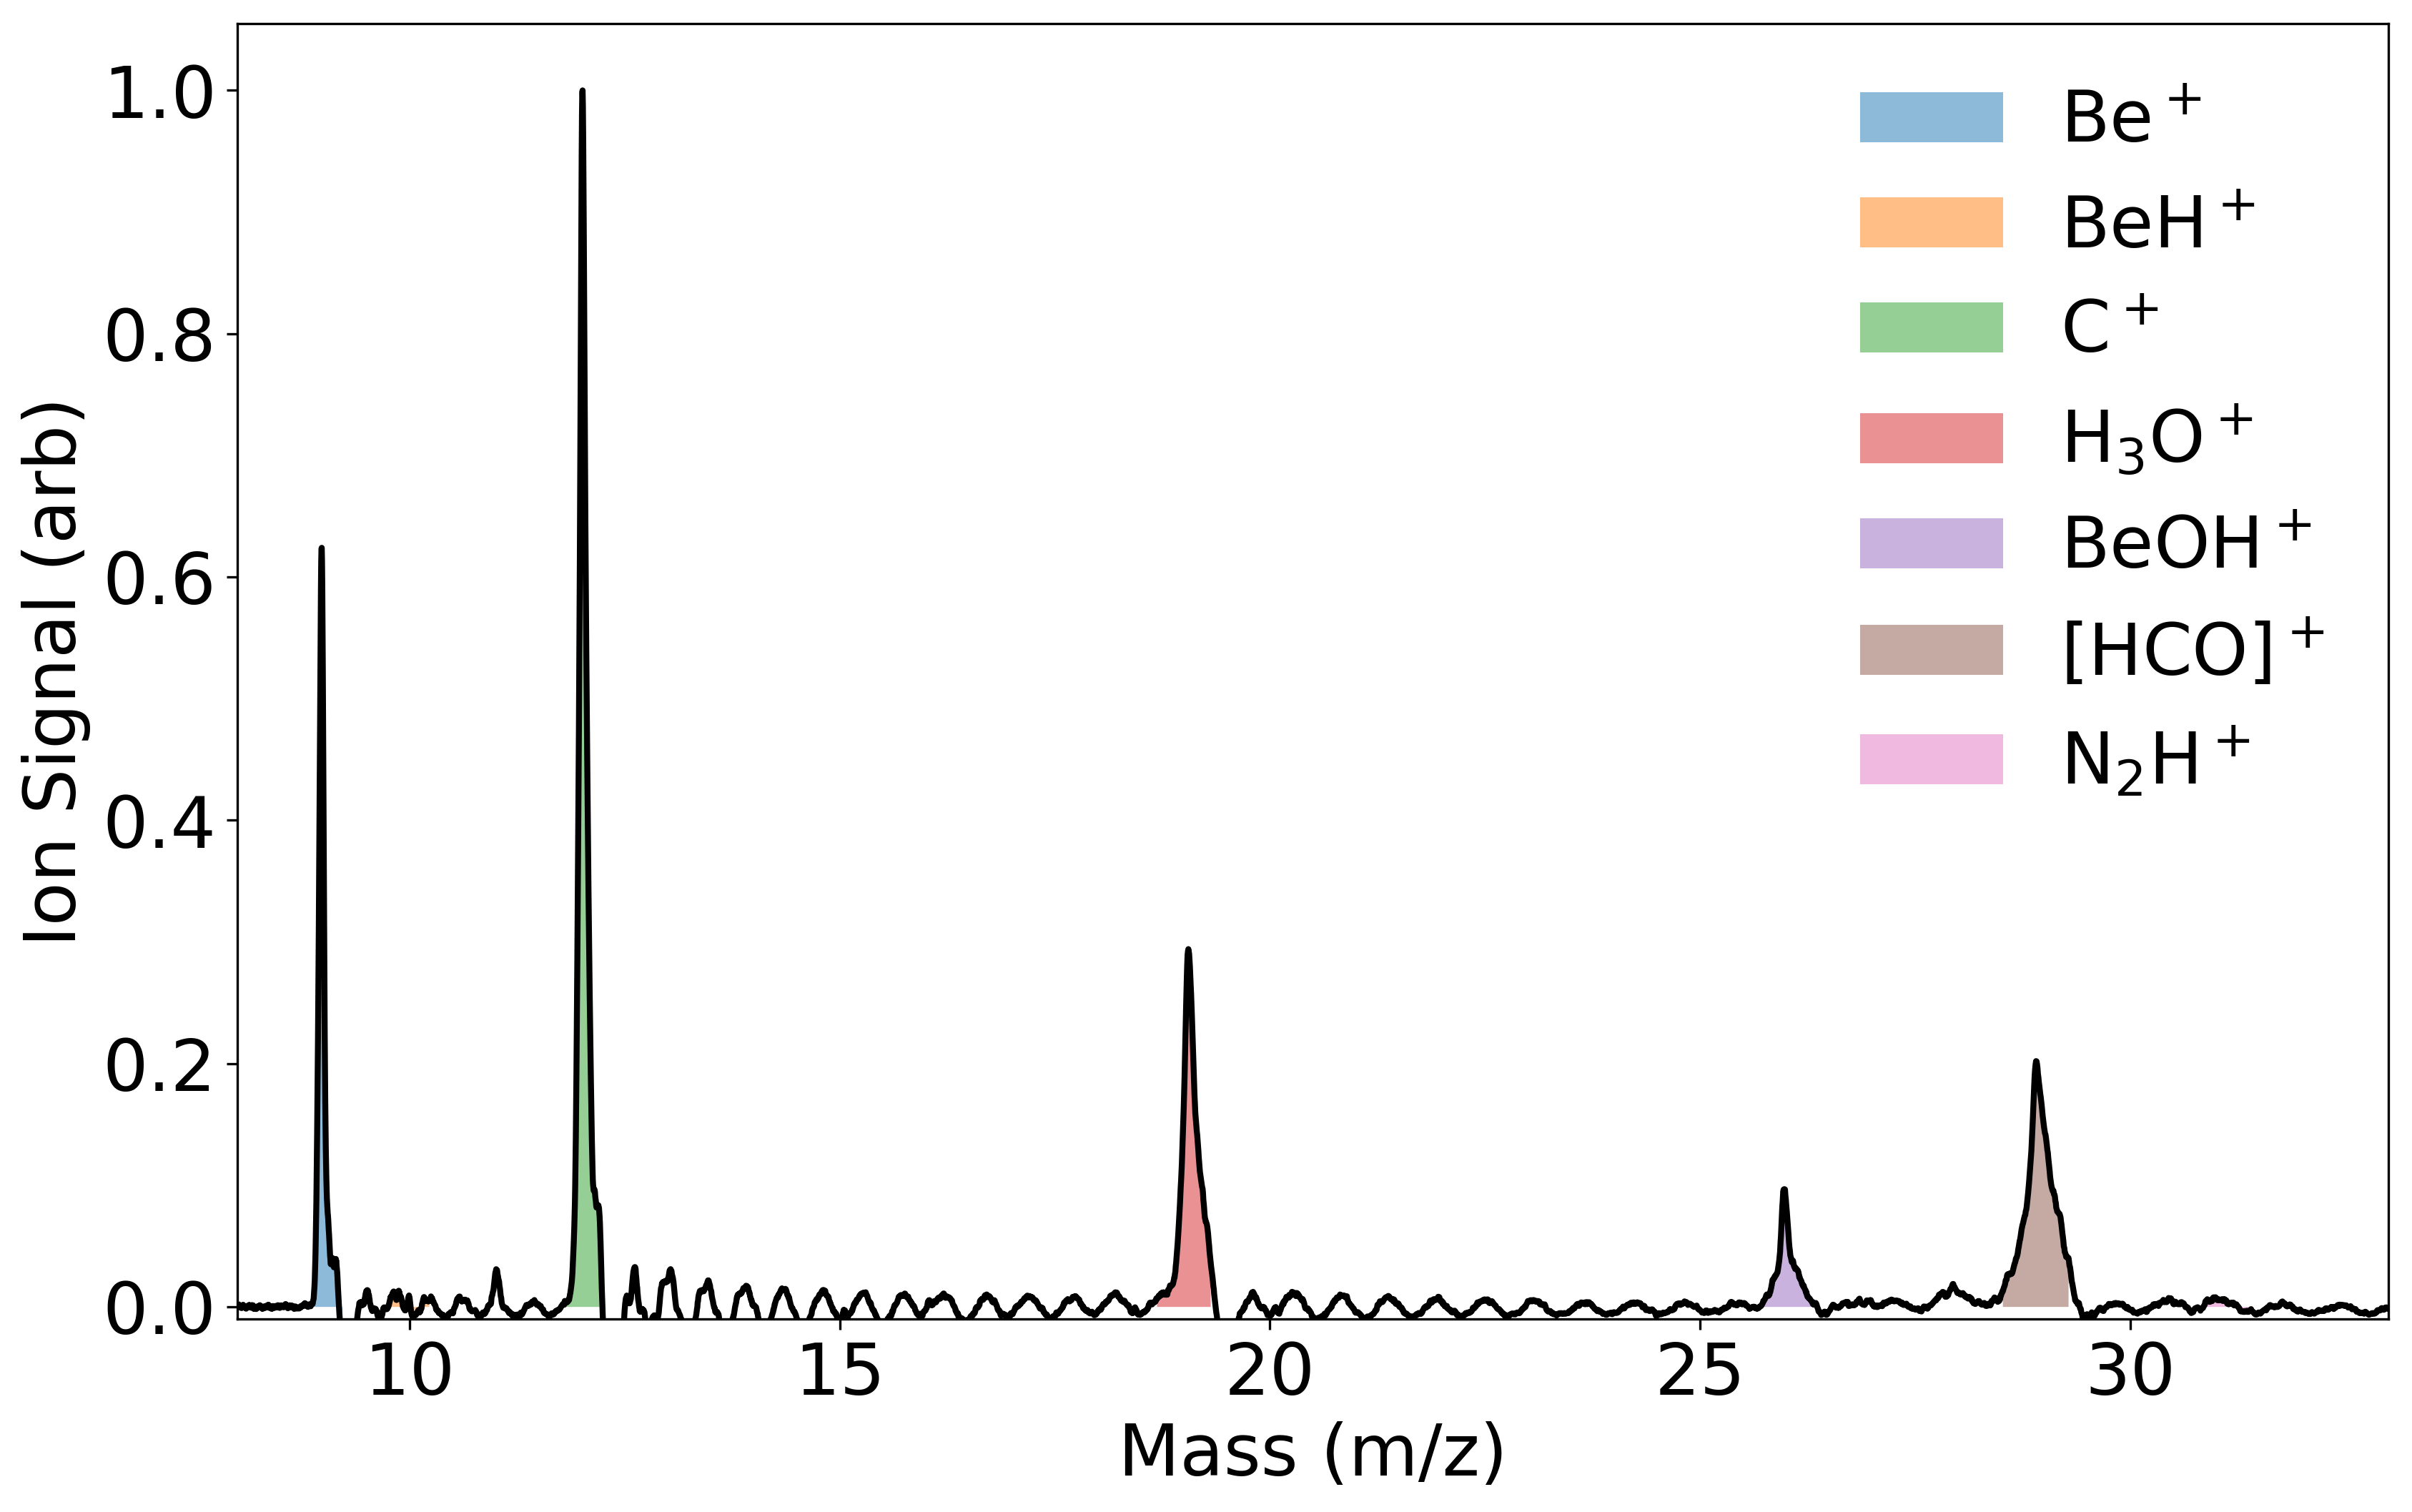
\includegraphics[width=0.8\textwidth]{images/C_H2O_CO_15N2.png}
	\caption{TOF trace of reaction products of \ce{Be+} and \ce{C+} after exposure to both water from the CBGB beam, and \ce{CO} (10 s) before titration with \ce{15N2} (10 s). There is a distinct lack of \ce{N2H+}, indicating full conversion of \ce{HOC+ -> HCO+}.} 
	\label{fig: CO N2 TOF}
\end{figure}

Integrated \ce{N2H+} signal was found to be below the threshold for a null signal, demonstrating both points that reaction \ref{r: HOC+CO->HCO} proceeds as expected, and experimental verification that reaction \ref{r: HCO+N2->NA} does not occur.

To determine the branching ratio, \ce{Be+} and \ce{C+} in the trap are exposed to the CBGB for 10 s, after which, the beam shutter in the beam path is closed. \ce{^15N2} is constantly introduced via leak valve to react with the \ce{HOC+}. Repeating this process over various densities of \ce{^15N2} allows us to determine the isomer branching ratio as well as the proton transfer rate constant. We expect the ratio of \ce{N2H+} and \ce{[HCO]+} to follow the form:
\begin{equation}
	\frac{\ce{^{15}N2H+}(t)}{\ce{^{15}N2H+}(t)+\ce{[HCO]+}(t)} = C \left( 1-e^{-k_{\ref{r: X+HOC->XH}} \rho t} \right)
	\label{eq: N2 asymptote}
\end{equation}
A fit performed on the data over various densities yields a rate constant of $k_{\ref{r: X+HOC->XH}} = ((6.6 \pm 1.0) \times 10^{-10})$ cm$^3$/s, and a final branching ratio of $\ce{HOC+}:\ce{HCO+} = 0.58 \pm 0.01$, in good agreement with the \ce{CO2} titration results.

\begin{figure}[H]
	\centering
	\makebox[\textwidth][c]{
		\begin{tabular}{cc}
			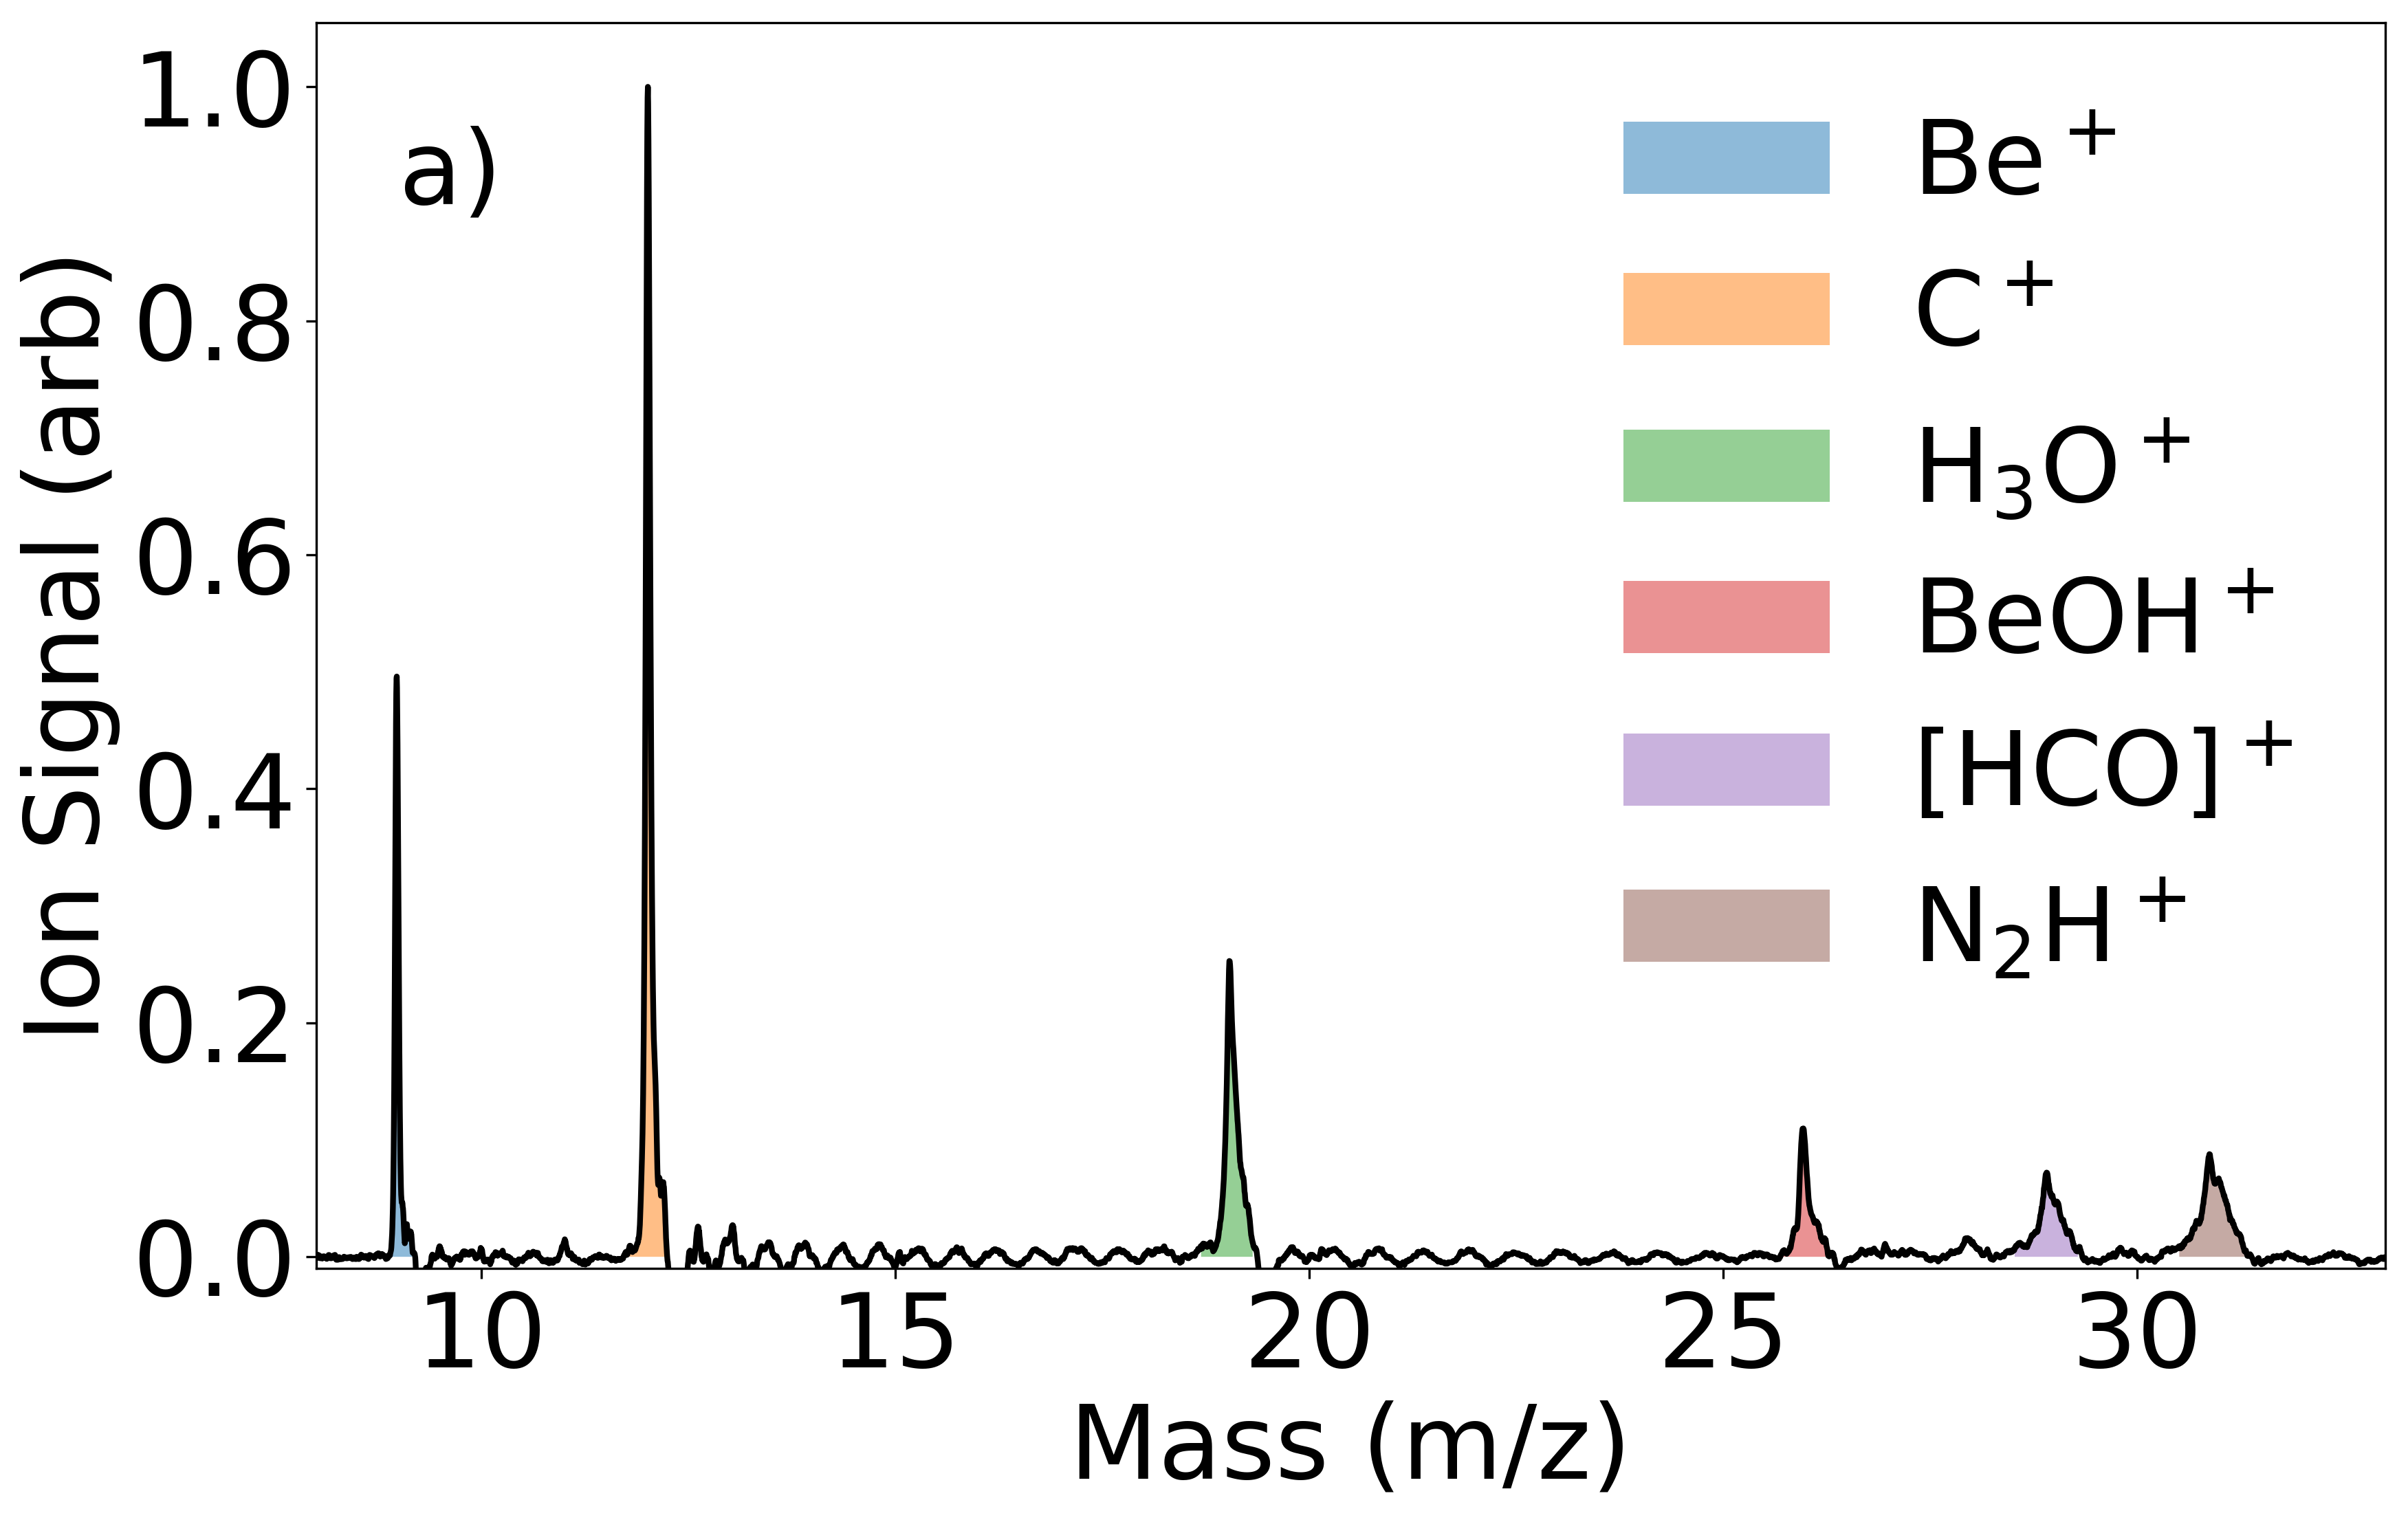
\includegraphics[width=0.5\textwidth]{images/C_H2O_15N2_small.png} &
			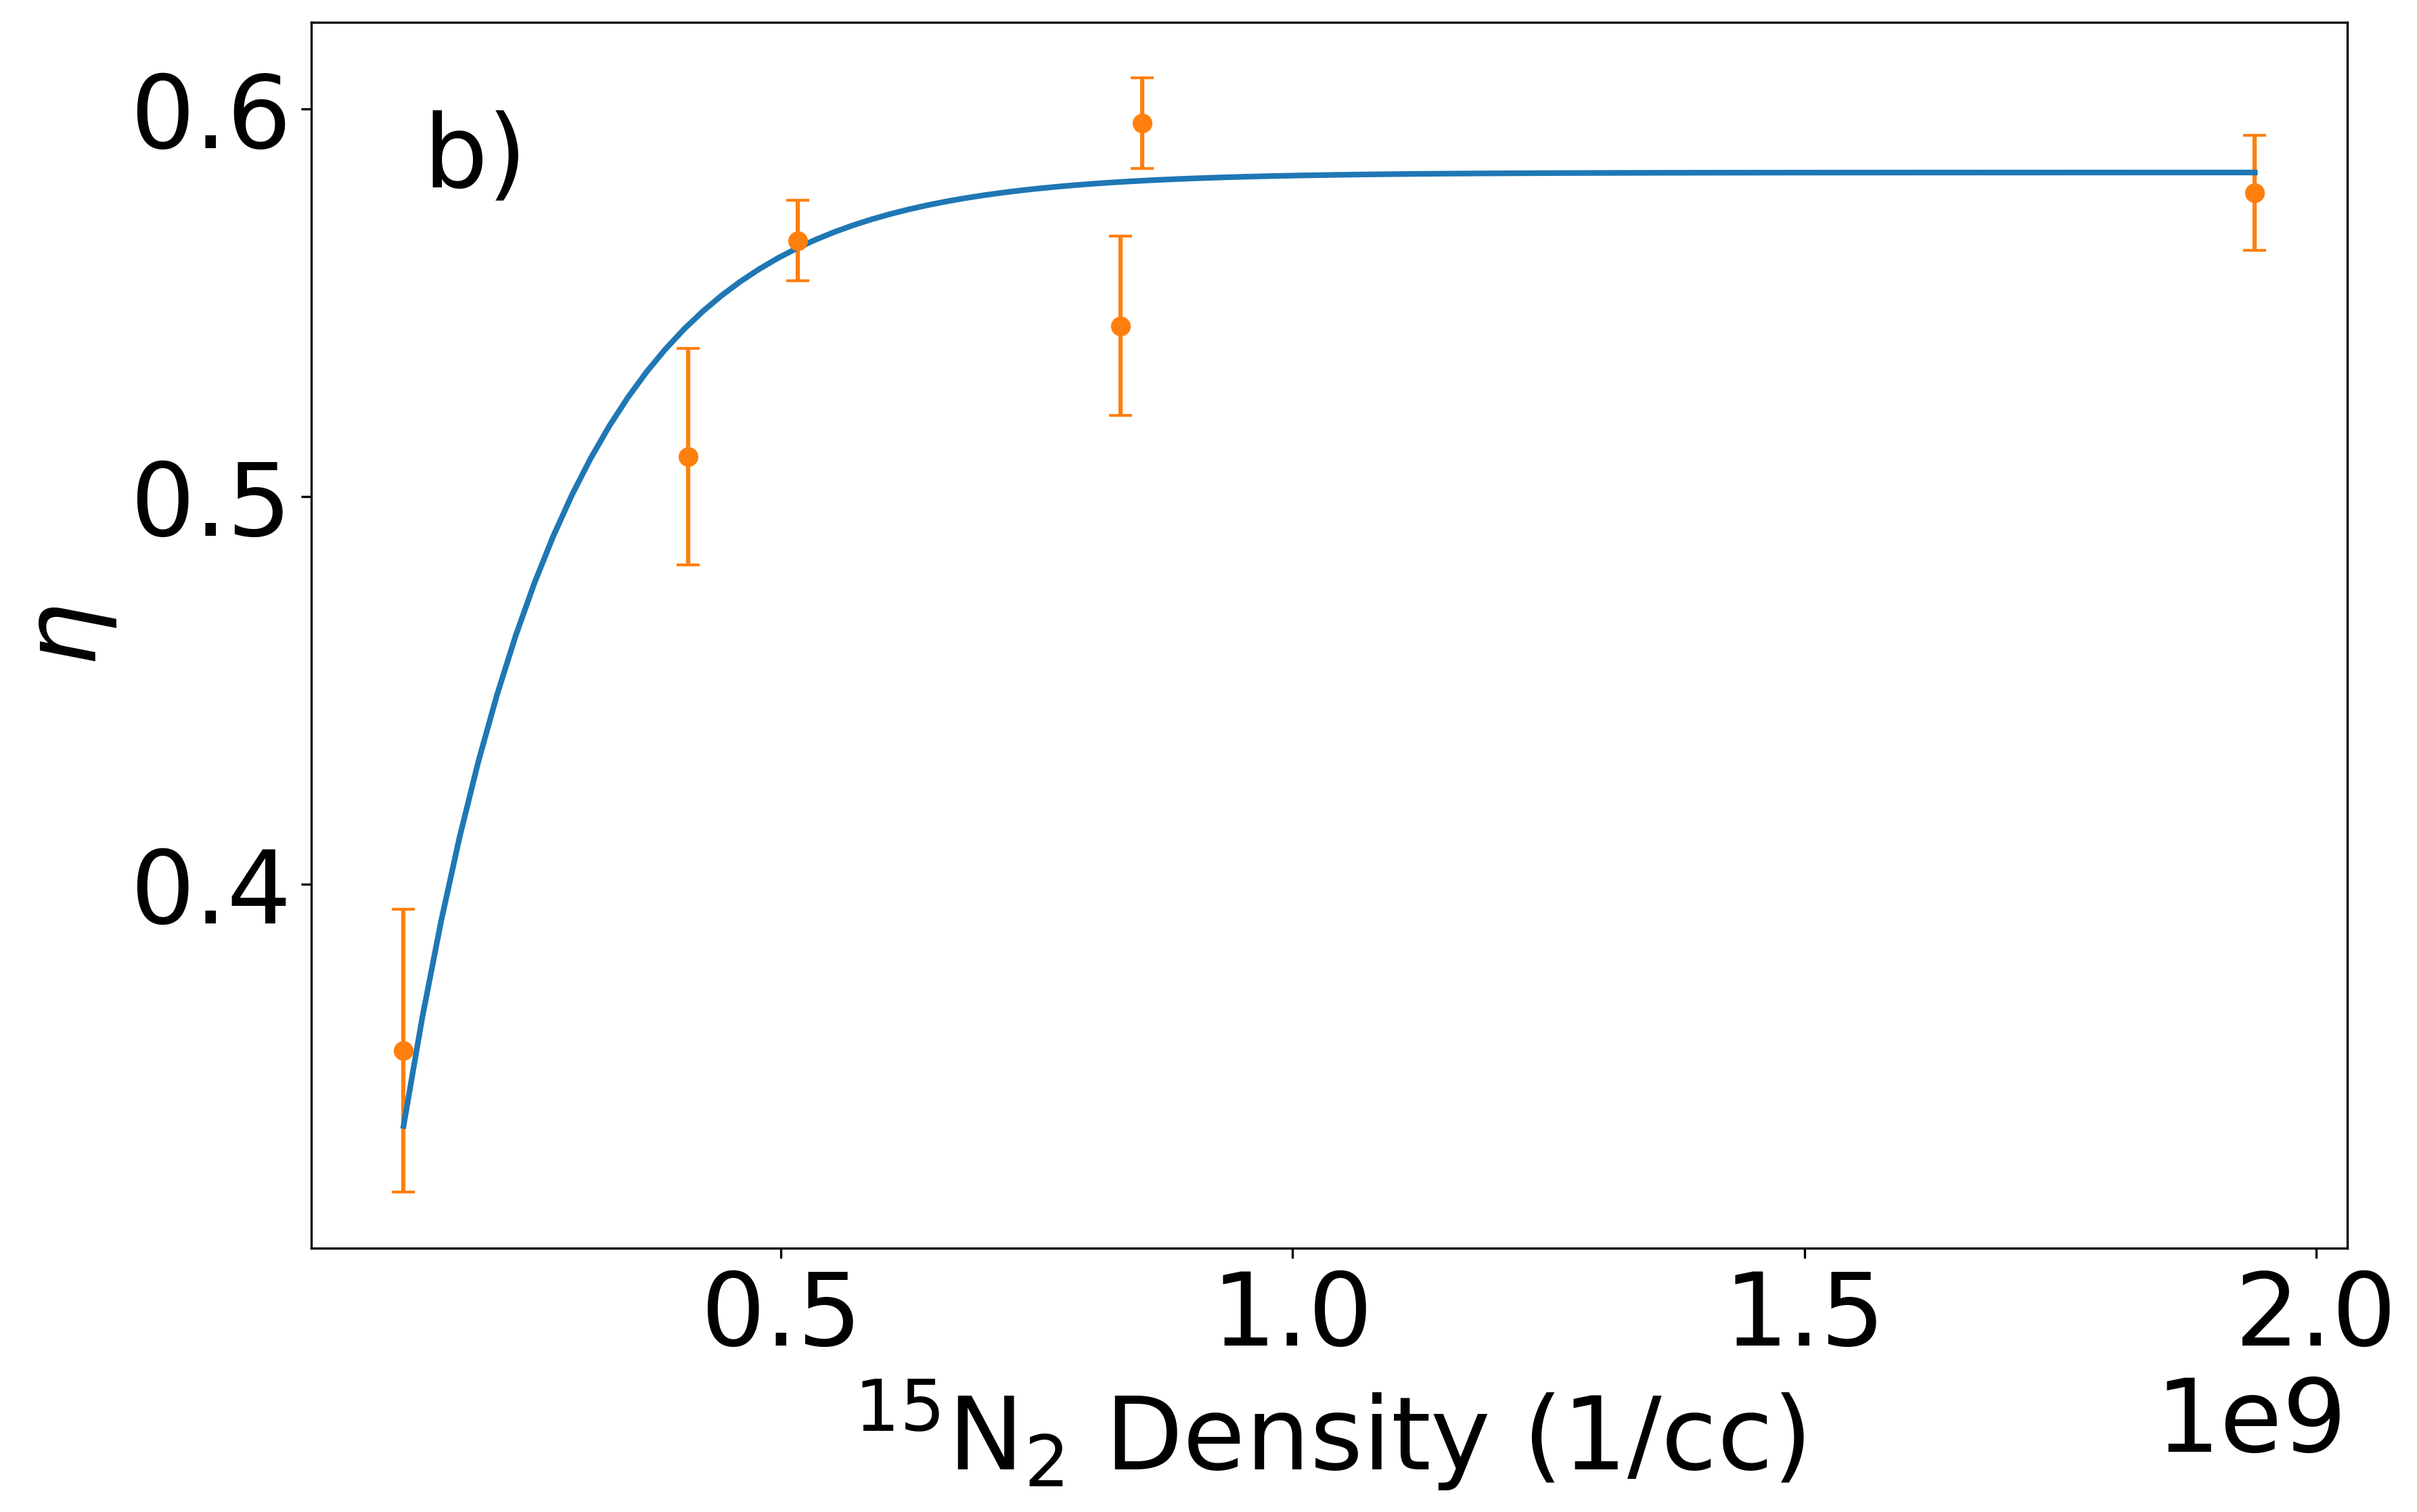
\includegraphics[width=0.5\textwidth]{images/N2_pressure_scan_small.png}
		\end{tabular}
	}
	\caption{a) Average of 10 TOF traces of \ce{Be+} and \ce{C+} exposed to water from the CBGB (10 s), then exposed to \ce{^15N2} from the leak valve (10 s) at a density of $1 \times 10^9$ cc$^{-1}$. b) The fraction of the titrated isomers, $\eta \equiv \ce{^{15}N2H+}/(\ce{^{15}N2H+}+\ce{[HCO]+})$, as a function of \ce{^15N2} density. Fitted parameters yield values $C = 0.58 \pm 0.01$, $k_{\ref{r: X+HOC->XH}} = ((6.6 \pm 1.0) \times 10^{-10})$ cm$^3$/s.}
	\label{fig: N2 pressure scan}
\end{figure}

To estimate a limit on the isomerization, we consider the titration reactions \ref{r: X+HOC->HCO} and \ref{r: X+HOC->XH}, where \ce{X = ^{15}N2} in the context that we can only determine the abundance of \ce{[HCO]+} and \ce{^{15}N2H+}. As a function of pressure, we cannot see reaction \ref{r: X+HOC->HCO}, but if it does contribute, we should see a discrepancy in the total rate constant, which we estimate to be Langevin: $k_L = 8.0 \times 10^{-10}$. This gives us a possible isomerization rate of 18\%, which then yield a branching ratio of 70:30.
%CO with beam
%
%k1: 7.39e-02, 5.88e-03
%k2: 2.23e-01, 2.02e-02
%C0: 8.25e-01, 7.11e-02
%mz290: 9.36e-02, 1.71e-02
%H3O0: 1.75e-02, 3.24e-03
%reduced chi squared: 1.31e+00
%k1 = 7.87e-09
%k2 = 2.38e-08
%k1 theory = 7.74e-09
%k2 theory = 5.15e-09

%beam 
%k1: 2.11e-02, 4.04e-03
%k2: 5.30e-02, 9.73e-03
%C0: 8.49e-01, 1.08e-01
%mz290: 3.52e-02, 9.54e-03
%H3O0: 9.63e-03, 3.12e-03
%reduced chi squared: 2.50e+00
%k1 = 9.14e-09
%k2 = 2.29e-08
%k1 theory = 7.74e-09
%k2 theory = 5.15e-09

\section{Conclusion}

Our experimental results yield directly measured branching ratios $(58\pm5):(42\pm5)$ and $(58\pm1):(42\pm1)$ via titration with \ce{CO2} and \ce{^15N2}, in good agreement with one another. As the results from the \ce{^15N2} titration were without unknown peaks, we take that to be the proper experimental result. Hua Guo provided theoretical support in performing QCT calculations on the \ce{C+ + H2O} reaction dynamics at collision temperatures around 10 K. They find an initial branching ratio of 97:3, with 19\% of their \ce{HCO+} above the self-isomerization barrier, this brings their ratio down to 74:26. Hua also provided us with calculations on the possible percentage of isomerization due to reaction \ref{r: X+HOC->HCO} where \ce{X -> ^15N2} to be 17\%, consistent with our experimental results. Adjusting our experimentally determined ratio by the possible isomerization, we yield a ratio result of $(70\pm1):(30\pm1)$, this is much closer to the QCT results.

These results are in contrast to the room temperature result of 86:14\cite{Love1987}, but in better agreement with phase space calculations claiming a branching ratio of 67:33 in the literature.\cite{DeFrees1984}